\documentclass[]{book}
\usepackage{lmodern}
\usepackage{amssymb,amsmath}
\usepackage{ifxetex,ifluatex}
\usepackage{fixltx2e} % provides \textsubscript
\ifnum 0\ifxetex 1\fi\ifluatex 1\fi=0 % if pdftex
  \usepackage[T1]{fontenc}
  \usepackage[utf8]{inputenc}
\else % if luatex or xelatex
  \ifxetex
    \usepackage{mathspec}
  \else
    \usepackage{fontspec}
  \fi
  \defaultfontfeatures{Ligatures=TeX,Scale=MatchLowercase}
\fi
% use upquote if available, for straight quotes in verbatim environments
\IfFileExists{upquote.sty}{\usepackage{upquote}}{}
% use microtype if available
\IfFileExists{microtype.sty}{%
\usepackage{microtype}
\UseMicrotypeSet[protrusion]{basicmath} % disable protrusion for tt fonts
}{}
\usepackage{hyperref}
\hypersetup{unicode=true,
            pdftitle={Open Science MOOC Book},
            pdfauthor={Open Science MOOC Team},
            pdfborder={0 0 0},
            breaklinks=true}
\urlstyle{same}  % don't use monospace font for urls
\usepackage{natbib}
\bibliographystyle{apalike}
\usepackage{longtable,booktabs}
\usepackage{graphicx,grffile}
\makeatletter
\def\maxwidth{\ifdim\Gin@nat@width>\linewidth\linewidth\else\Gin@nat@width\fi}
\def\maxheight{\ifdim\Gin@nat@height>\textheight\textheight\else\Gin@nat@height\fi}
\makeatother
% Scale images if necessary, so that they will not overflow the page
% margins by default, and it is still possible to overwrite the defaults
% using explicit options in \includegraphics[width, height, ...]{}
\setkeys{Gin}{width=\maxwidth,height=\maxheight,keepaspectratio}
\IfFileExists{parskip.sty}{%
\usepackage{parskip}
}{% else
\setlength{\parindent}{0pt}
\setlength{\parskip}{6pt plus 2pt minus 1pt}
}
\setlength{\emergencystretch}{3em}  % prevent overfull lines
\providecommand{\tightlist}{%
  \setlength{\itemsep}{0pt}\setlength{\parskip}{0pt}}
\setcounter{secnumdepth}{5}
% Redefines (sub)paragraphs to behave more like sections
\ifx\paragraph\undefined\else
\let\oldparagraph\paragraph
\renewcommand{\paragraph}[1]{\oldparagraph{#1}\mbox{}}
\fi
\ifx\subparagraph\undefined\else
\let\oldsubparagraph\subparagraph
\renewcommand{\subparagraph}[1]{\oldsubparagraph{#1}\mbox{}}
\fi

%%% Use protect on footnotes to avoid problems with footnotes in titles
\let\rmarkdownfootnote\footnote%
\def\footnote{\protect\rmarkdownfootnote}

%%% Change title format to be more compact
\usepackage{titling}

% Create subtitle command for use in maketitle
\providecommand{\subtitle}[1]{
  \posttitle{
    \begin{center}\large#1\end{center}
    }
}

\setlength{\droptitle}{-2em}

  \title{Open Science MOOC Book}
    \pretitle{\vspace{\droptitle}\centering\huge}
  \posttitle{\par}
    \author{Open Science MOOC Team}
    \preauthor{\centering\large\emph}
  \postauthor{\par}
      \predate{\centering\large\emph}
  \postdate{\par}
    \date{2019-08-01}

\usepackage{booktabs}
\usepackage{amsthm}
\makeatletter
\def\thm@space@setup{%
  \thm@preskip=8pt plus 2pt minus 4pt
  \thm@postskip=\thm@preskip
}
\makeatother

\begin{document}
\maketitle

{
\setcounter{tocdepth}{1}
\tableofcontents
}
\hypertarget{preface}{%
\chapter*{Preface}\label{preface}}
\addcontentsline{toc}{chapter}{Preface}

\textbf{OPEN SCIENCE MOOC}

\textbf{\emph{We want to help make open the default setting for all global research.}} \emph{We want to develop a peer-to-peer, value-based community that works towards better science for society. Our ultimate goal is to help make `open' the default setting for all global research, through creating and connecting a welcoming and supporting community, based around good tools, teachers, and role models, fundamentally built upon a solid values-based foundation of freedom and equitable access to research.}

\hypertarget{warning---tentative-book}{%
\section*{Warning - Tentative book}\label{warning---tentative-book}}
\addcontentsline{toc}{section}{Warning - Tentative book}

As of now, this book is purely done out of free time here and there and serve only as a proof of concept to provide a portable/downloadable format for the Open Science MOOC content available on Eliademy. This is an example of using the bookdown package to write the Open Science MOOC Book that will link all modules and supplemental material.

\hypertarget{rationale}{%
\section*{Rationale}\label{rationale}}
\addcontentsline{toc}{section}{Rationale}

Research is getting a global makeover, in part thanks to the power of the internet and the tools it provides for us, and in part due to a growing call for accountability (e.g., reproducibility and data provenance) in research. Global policies are emerging at different levels that include some aspect of Open Research, Open Scholarship, or Open Science, and inclusive of all research disciplines. But our universities are often letting us down, and they are not teaching us the knowledge, tools and skills we need to do research effectively in the 21st century.

Open Science is about increased rigour, accountability, reproducibility for research. It is based on the principles of inclusion, fairness, equity, and sharing. Open Science can be viewed as research simply done properly, and it extends across the Life and Physical Sciences, Engineering, and Mathematics, to Social Science and Humanities.

This MOOC is designed to help equip students and researchers with the skills they need to excel in a modern research environment. It brings together the efforts and resources of hundreds of researchers and practitioners who have all dedicated their time and experience to create a community platform to help propel research forward.

The content of this MOOC will be distilled into 10 core modules. Each module will comprise a complete range of resources including videos, research articles, dummy datasets and code, as well as tasks to complete as individuals or groups.

The MOOC will be hosted through an open source provider. We expect that in the future different systems of certification will be developed, including completion badges. We also intend to build a forum for the open discussion of the MOOC and any relevant topics.

\emph{Disclaimer:} We, the contributors, are fully aware that there is no magic one size fits all solution when it comes to implementing Open Science philosophies and best practices, especially when covering all research disciplines. However, we also believe that we should not limit ourselves from the onset, just because pragmatic solutions may not exist today for certain disciplines. We aim to set a highly inclusive standard, fully accepting the risk that for some disciplines this strategy may not be fully appropriate. Through that failure, we hope that you, the course users, will join us as course contributors and help us co-create bespoke solutions to your discipline based on principles of transparency, provenance, reproducibility and reuse of knowledge.

\hypertarget{module1}{%
\chapter{Open Principles}\label{module1}}

\emph{Estimated time to complete: 60 minutes}

\emph{Estimated saving time: A lot}

\hypertarget{table-of-contents}{%
\section*{Table of Contents}\label{table-of-contents}}
\addcontentsline{toc}{section}{Table of Contents}

\begin{itemize}
\tightlist
\item
  \protect\hyperlink{introduction}{Introduction}

  \begin{itemize}
  \tightlist
  \item
    \protect\hyperlink{who_for}{Who is this module for?}
  \item
    \protect\hyperlink{objectives}{Specific learning objectives for this module}
  \end{itemize}
\item
  \protect\hyperlink{what_is}{What is Open Science?}

  \begin{itemize}
  \tightlist
  \item
    \protect\hyperlink{values}{Community values in Open Science}
  \item
    \protect\hyperlink{cultures}{History of Open Science and Open Cultures}
  \item
    \protect\hyperlink{interpretation}{Differences in understanding and interpretation}
  \item
    \protect\hyperlink{network_effects}{Open Scientists share objects to gain network effects for their work}
  \end{itemize}
\item
  \protect\hyperlink{principles}{Principles of Open Science}
\item
  \protect\hyperlink{dimensions}{The different dimensions of Open Science}
\item
  \protect\hyperlink{impacts}{How Open Science impacts you; \textbf{TASK 1}}

  \begin{itemize}
  \tightlist
  \item
    \protect\hyperlink{evaluation}{Changes in research evaluation}
  \item
    \protect\hyperlink{career}{Potential impact on your career}
  \item
    \protect\hyperlink{profile}{Creating your digital profile; \textbf{TASK 2}}
  \end{itemize}
\item
  \protect\hyperlink{barriers}{Barriers and limitations in Open Science}

  \begin{itemize}
  \tightlist
  \item
    \protect\hyperlink{tradition}{Moving away from tradition and the status quo}
  \end{itemize}
\item
  \protect\hyperlink{reproducible}{Open Science and reproducible research}
\item
  \protect\hyperlink{workflow}{Making Open Science part of your daily research workflow}
\item
  \protect\hyperlink{future}{Where to go from here}
\item
  \protect\hyperlink{development_team}{Development Team}
\end{itemize}

\textbf{BEFORE YOU START}

\begin{quote}
Science is everywhere, science is all around us. This is your last chance. After this there is no turning back. You take the \href{https://www.elsevier.com/about/open-science}{blue pill}, the story ends, you wake up in your bed, and believe whatever you want to believe. You take the \protect\hyperlink{Introduction}{red pill}, you stay in Wonderland, and we show you how deep the rabbit hole goes. (Fishburne, 1999)
\end{quote}

Did you know that the Internet and the World Wide Web were both originally designed for research purposes? Researchers wanted a fast, easy, and low-cost way for sharing data with each other, and hence the Internet was born. Now, the Internet dominates almost all aspects of our daily lives, and yet has somehow deviated from this original purpose. Now, research seems to have gone almost backwards compared to every other enterprise - Open Science is the movement to bring modern research back into line with this original digital intent, while reasserting fundamental scientific principles back to the endeavour.

Did you also now that this is so important, that it is even in the \href{http://www.un.org/en/universal-declaration-human-rights/}{United Nations Declaration on Human Rights}?

\begin{quote}
\begin{enumerate}
\def\labelenumi{(\arabic{enumi})}
\tightlist
\item
  Everyone has the right freely to participate in the cultural life of the community, to enjoy the arts and to share in scientific advancement and its benefits.
\end{enumerate}
\end{quote}

\begin{quote}
\begin{enumerate}
\def\labelenumi{(\arabic{enumi})}
\setcounter{enumi}{1}
\tightlist
\item
  Everyone has the right to the protection of the moral and material interests resulting from any scientific, literary or artistic production of which he is the author.
\end{enumerate}
\end{quote}

You have probably landed here because you have a nagging feeling that something about the way modern research is conducted and shared is not quite right. This module will hopefully shed some light on those feelings, and help you to understand the state of the present system, and its discord within intrinsic human and scientific values and principles. This is the start of your own journey to become an \emph{awesome} researcher and a \emph{champion} in your field. Hopefully, by being here, we can all work together to empower individuals and communities to make changes to research cultures that we haven't even imagined yet!

\hypertarget{introduction}{%
\section{Introduction }\label{introduction}}

Welcome to Module 1 of the Open Science MOOC: Open Principles. This is the first of 10 core modules to give you a solid grounding in all things Open Science. This module has been developed \href{"</a></strong></p>

You, yes you, are in the middle of a profound global scientific revolution. To innovate in a field frequently implies moving against prevailing trends, structures, and cultural inertia. \textbf{Open Science} is no different. The fact that \emph{you} are here, reading this now, means that you probably have an interest in the impact that Open Science can have on improving research cultures, and have noticed that something is not quite right about the ``status quo'' in modern research.

This module will introduce to you the guiding principles, values, and practices of `Open Science', some of the potential barriers to these, and the positive impact that integrating openness into your daily research work can have on you. This module is not designed to be a `one size fits all' approach, but rather a foundational plan that incorporates questions around the varying and dynamic dimensions, interpretations, and goals of Open Science across different communities.

Image license: CC0 1.0 Universal; Patrick Hochstenbach \textless{}a href=``\url{https://twitter.com/hochstenbach}'' target=""

\hypertarget{who-is-this-module-for}{%
\subsection{Who is this module for? }\label{who-is-this-module-for}}

Designed primarily for students and researchers at the graduate and undergraduate level, this module also serves as training material for postdocs and more senior researchers. We want to help make openness universal and for all, not just a select few. This aims to be a cross-disciplinary module covering all research branches, including Engineering, Medicine, Biosciences, Mathematics, Social Sciences, Humanities, and the Arts.

We have set a highly inclusive standard, and right from the very beginning have had people from across the \emph{whole} spectrum of scholarly research, and related disciplines like tech, publishing, and librarianship, involved in developing and scoping the project. We use the term `Open Science' given that this seems to be the phrase that global changes are coalescing around; while recognising that terms such as `Open Research' or `Open Scholarship', although less widely used, might capture a bit better what our intention is here.

Therefore, irrespective of your background \textbf{you are very much welcome here}.

\begin{quote}
``Open Science describes the practice of carrying out scientific research in a completely transparent manner, and making the results of that research available to everyone. Isn't that just `science'?!'' - Mick Watson-- \href{"</a></strong></p>
\end{quote}

Melanie Imming, \& Jon Tennant. (2018, June 8). Sticker Open Science: just science done right. Zenodo. https://zenodo.org/record/1285575\#.XDebSM17lPY

\hypertarget{specific-learning-objectives-for-this-module}{%
\subsection{Specific learning objectives for this module }\label{specific-learning-objectives-for-this-module}}

\begin{enumerate}
\def\labelenumi{\arabic{enumi}.}
\item
  Understand the ethical, legal, social, economic, philosophical, and research impact arguments for and against Open Science.
\item
  Set up a personal profile for defining your impact: Measure the social and academic attention for the full range of your research processes and outputs.
\end{enumerate}

\hypertarget{what-is-open-science}{%
\section{What is Open Science? }\label{what-is-open-science}}

\begin{quote}
None of us is as smart as all of us. - Kenneth H. Blanchard.
\end{quote}

The term `Open Science' has not yet a universally accepted definition, but usually refers to one core theme: \textbf{Increasing knowledge availability as a public good}, typically with critical research principles such as credibility, reproducibility, and verifiability included in some combination. Many other terms are being used synonymously with Open Science, such as Open Research, Open Scholarship, Science 2.0, and eScience.

Throughout this MOOC, we consider `Open Science' to be fully inclusive of all of these terms, all scholarly research disciplines, and to reflect the wider process of organised knowledge creation \href{"</a></strong></p>

Ironically, the only current peer-reviewed research article to systematically attempt to define Open Science is paywalled, so we do not include it here. Sigh. (DOI, for those interested: 10.1016/j.jbusres.2017.12.043)

\begin{quote}
\href{https://www.fosteropenscience.eu/}{FOSTER} defines Open Science as: ``The movement to make scientific research, data and dissemination accessible to all levels of an inquiring society.''
\end{quote}

Open Science can broadly be viewed as a way of enhancing scientific progress through sharing of knowledge and methods, wider collaboration, and increased rigour and is indirectly already postulated as part of our/researchers' collective core values and \textbf{Good Scientific Practices}. Research can only thrive if it is shared and built upon.

Often, the usage of Open Science seems to be based around three core things: \emph{Processes} (e.g., collaboration, reproducibility), \emph{Products} (e.g., Open Data, Open Materials), and \emph{Values} (e.g., freedom, equity). This seems to form a chain reaction and positive feedback loop, where values drive a particular process, which in turn scopes the products of research.

\hypertarget{community-values-in-open-science}{%
\subsection{Community values in Open Science }\label{community-values-in-open-science}}

The values inherent to Open Science have again not yet been rigorously defined or accepted by the global research community. However, there are a number of inherent values that come up time and time again in discussions of openness. These include: \textbf{diversity, inclusivity, fairness, equity, social behaviour, accountability, ethics and responsibility.}

Now, these are not necessarily values that are exclusive to scientific research, and are more human in nature. This is critical, as it helps to frame Open Science as an inherent human nature, and thus amplifies its social importance and imperative.

\begin{quote}
How do we use Open Science approaches in the context of retooling our institutions to benefit actual living and breathing humans (scientists and nonscientists)? How can we use Open Science to enable as many people who have the interest and talent to pursue science for it's own sake and to generate knowledge that is broadly useful for society, and not just elite institutions, venture capital firms or global megacorporations? - Alex Lancaster \href{http://ronininstitute.org/open-science-and-its-discontents/}{(source)}.
\end{quote}

\begin{quote}
I am, somehow, less interested in the weight and conviolutions of Einstein's brain than in the near certainty that people of equal talent have lived and died in cotton fields and sweatshops. - Stephen Jay Gould.
\end{quote}

Part of the mission for the Open Science MOOC is to help to achieve this alignment as part of a grassroots movement.

Therefore, some of the key, value-based goals of the Open Science community include:

\begin{itemize}
\item
  \textbf{Freely available access to all outputs of the whole research process;}
\item
  \textbf{Equity and inclusive participation in research;}
\item
  \textbf{Diverse and creative interpretations of scientific results;}
\item
  \textbf{Rigorous, transparent, and responsible evaluation of research processes and outcomes;}
\item
  \textbf{Collaborative re-use of research outcomes, reducing costs, waste and redundancy;}
\item
  \textbf{Comprehensive research practices incentivised through more diverse reward systems;}
\item
  \textbf{Accelerated research discovery, innovation and public impact;} and
\item
  \textbf{Increasing reproducibility of research results, enhancing trustability and integrity.}
\end{itemize}

If these things are all true, then we have to ask of ourselves: \emph{Why isn't all publicly-funded science practised this way?}

It seems that Open Science is often communicated as an \emph{alternative} to many modern or traditional scientific methods. We argue that Open Science is an \emph{enhancement} of the traditional process, using new knowledge, skills, and technologies to improve how the process and outputs of research are communicated. It is based on fundamental human values around \textbf{inclusivity}, \textbf{freedom}, and \textbf{equity}, embedded as foundational elements to the research process, rather than as an afterthought. These human values are what distinguish `Open' science from much of the way modern research is viewed and practised. We also believe that virtually everyone who comes into research already has these fundamental values as part of who they are. However, often they become divergent from the way in which the academic system forces them to work. We want to change that.

The foundational elements of traditional research communication, peer-reviewed research articles, act as an important mechanism to summarise and communicate research. Open Science helps to make research articles more rigorous, verifiable and reliable. This helps to enhance public trust in the scientific community and endeavour. In modern society, this has never been more important.

\begin{quote}
Open Science is subject to the most rigorous peer review because the process never ends. - \href{"</a></strong></p>
\end{quote}

Perhaps one of the most important aspect of the Open Science movement in recent years has been the drive behind the liberation of research papers from behind paywalls to be freely available to anyone; also known as Open Access. This has largely been based on the principle that humans deserve to have access to scientific knowledge, and benefit from that.

Number of articles (A) and proportion of articles (B) with OA copies, estimated based on a random sample of 100,000 articles with Crossref DOIs. Piwowar et al. (2018)

Still today (2018), most research papers remain locked behind expensive paywalls, critical research data remains hidden away on hard-drives, methods remain often scantly documented, research results cannot be reproduced, and researchers are often evaluated on senseless criteria such as the journal impact factor. These are just some examples of typical practices that contribute to what might be viewed as `closed science'; or bad (unethical) scientific practices.

Open Science is about changing these research practices through a cultural/paradigm shift. This shift in research culture is often referred to as the \href{https://www.force11.org/group/scholarly-commons-working-group}{\textbf{Scholarly Commons}}, which seeks to explore and redefine what a modern scholarly communication ecosystem should look like.

Accomplishing a cultural shift on a global scale is far from easy. Fundamentally, it is usually mainly done through the spread of shared cultural norms and values that are interpreted and celebrated in hundreds of local institutions: in your department, school, laboratory, university, professional association, publishing effort, open software platform developer company, or funding agency. It is a complex, multi-dimensional paradigm to comprehend. Each of these organizations fits itself into the cultural practices that members decide will work best for them to become active in performing the cultural work of Open Science. Culture change \emph{must} start from the ground up. Open Science principles illuminate this ground.

The power of modern Web technologies enables instantaneous sharing and global collaboration in an unrestricted fashion. The digital era is transforming the way in which research is performed, and the limitations on distribution of the print era are largely gone (at least in theory). With this, new issues arise including the complexities of knowledge capture and communication. The framing of these complexities as a `Commons' integrates the political, social, economic, and philosophical dimensions around knowledge generation and sharing.

Open Science gives rise to a new set of standards, tools, principles, and practices to revolutionise the way we perform and disseminate research knowledge. And we are going to need all of this, if we want to help shape our world for the better.

For example, the United Nations has recently set a number of critical Sustainable Development Goals.

UN Sustainable Development Goals

The question to you is, \emph{do you believe that science can help progress towards reaching these goals?} Hopefully, your answer is a resounding \textbf{YES}. But if so, you must also acknowledge that much of the way we often currently practise science in a `closed' manner means that we are not doing the best that we can to achieve this. Open Science can be a cultural shift that helps to make the world a better place.

\hypertarget{history-of-open-science-and-open-cultures}{%
\subsection{History of Open Science and Open Cultures }\label{history-of-open-science-and-open-cultures}}

In the 1660s, Robert Boyle, the ``father of chemistry,'' broke with the practices of alchemy in his early writings, e.g., \href{https://en.wikipedia.org/wiki/The_Sceptical_Chymist}{The Sceptical Chymist}, and promoted open experimentation (following Roger Bacon's model). Previously, alchemists occulted their methods and their knowledge died with them. What might have been called ``open alchemy'' became ``natural philosophy'' and then ``science.'' \textbf{Science was born open}.

The commitment to opening science to help make it more transparent and accessible is nothing new. For some historians of science openness marks the beginning of science itself: with the printing press, the rise of publication markets and empirical methods in the early modern period came both the professionalization of scientists and the institutionalization of the Academies \href{https://ssrn.com/abstract=2209188}{(David 2008)}.

The earliest form of Open Science can perhaps trace its origins back the 17th century, and the origins of the academic journal, such as the \href{https://en.wikipedia.org/wiki/Philosophical_Transactions_of_the_Royal_Society}{Philosophical Transactions of the Royal Society}. \emph{Transactions} collected and disseminated a broad range of observations and experiment descriptions and spread the work of the Invisible College, the informal gathering of natural philosophers at Oxford and elsewhere. Publication of scientific ``news'' was also catalysed by an increasing demand for the wider dissemination of scientific knowledge with the wider public. However, the origins can probably go back even further to the very birth of scholarly practices. Much of what we know about our world and universe has foundations in fundamental openness, from evolution and the origin of species, through to gravity and the origins of stars.

The intersections of Open Science and Open Culture, by Katja Mayer (CC BY)

Although difficult to pin down exactly, the origins of what many call the modern `Open Science movement' were probably catalysed by increasing frustration, debate, and distress regarding the impacts of `closed science' (e.g., barriers such as subscription paywalls) and commercialisation of knowledge dissemination by corporate publishers. Indeed, one of the rallying cries of the Open Science movement is that taxpayers who have already paid to fund research should not be having to pay again to read the results of it.

The term ``Open Science'' itself appears to have been coined by \href{https://en.wikipedia.org/wiki/Open_science\#Coining_of_phrase_\%22OpenScience\%22}{Steve Mann in 1998}. Today's ``Open Science movement'' though probably dates back about 30-40 years, and takes inspiration both from the history of ``open source'' and the ``free software movement'' \href{https://www.twobits.net/pub/Kelty-TwoBits.pdf}{(Kelty 2008)} and the ideas developed for research collaboration in the context of ``e-science''. At a first glance these approaches refer mainly to the technological dimension of opening up science by creating necessary tools and infrastructures. Opening up science often takes the form of a technological liberation and change of techniques in respective discourses. However, keeping in mind that science and technology ``are politics by other means'' (Bruno Latour, 1978) - offering other means of power - it is vital to turn to the embedded politics of Open Science and its precursors.

In the last two decades, there has been an explosive growth in the development of different aspects of scholarly infrastructure - the core, underpinning aspects of a well-functioning research machine. Much of this is a blend of non-profit and commercial services, which are now variably integrated, but has created a strange and complex new system of ways to perform and communicate research. It is difficult to cast judgement on `for-profit' versus `not-for-profit' entities with respect to openness in a simple binary way. For example, for-profit entities like \href{https://publons.com/}{Publons} and \href{https://figshare.com/}{Figshare} were important in catalysing changes in crediting peer review and Open Data respectively; while not-for-profits like the \href{https://www.scientificamerican.com/article/open-access-to-science-un/}{American Chemical Society} have actively lobbied against progressive changes around Open Science.

From this, what might (hopefully) be becoming a little more clear is that Open Science is about systemic change. It challenges the way research is conducted, at a practical and cultural level, the way it is evaluated, and the ways in which scientific knowledge is disseminated and integrated into the functioning of society. Much of this is ingrained into research culture through self-reinforcing local governance systems, which are often imposed through external capitalist pressure. For example, the `\emph{publish or perish}' mantra is a direct consequence of these pressures, which in turn are linked to the evolving \href{https://opinionator.blogs.nytimes.com/2009/03/08/neoliberalism-and-higher-education/}{neoliberal agenda} imposed by modern research institutes.

If the above makes sense to you, it might seem like Open Science is in almost direct conflict with a capitalistic culture. This conflict is not new to science. In the 1940s, famed sociologist Robert Merton articulated some of the results of his sociology of science research as a set of four norms: principles that described the underlying ethos of science. Each of these norms is sharply divergent to how a free marketplace operates. You can read about the norms \href{https://en.wikipedia.org/wiki/Mertonian_norms}{here}. One of Merton's norms was ``communism,'' (this is sometimes re-worded as ``communalism''):

\begin{quote}
``\,`Communism,' in the nontechnical and extended sense of common ownership of goods, is a second integral element of the scientific ethos. The substantive findings of science are a product of social collaboration and are assigned to the community. They constitute a common heritage in which the equity of the individual producer is severely limited.'' - Originally published as ``Science and Technology in a Democratic Order,'' \emph{Journal of Legal and Political Sociology}, and then later published as ``Science and Democratic Social Structure,'' in Robert K. Merton, \href{https://en.wikipedia.org/wiki/Social_Theory_and_Social_Structure}{\emph{Social Theory and Social Structure}}. A link to a summary version can be found \href{https://www.collier.sts.vt.edu/5424/pdfs/merton_1973.pdf}{here}.
\end{quote}

The other three \href{https://scienceblogs.com/ethicsandscience/2008/01/29/basic-concepts-the-norms-of-sc}{norms} are:

\begin{itemize}
\tightlist
\item
  Universalism: That researchers should be concerned with the content of claims, not with who made them;
\item
  Disinterestedness: That researchers are in this for more than just personal gain; and
\item
  Organised skepticism: That anyone can potentially advance knowledge claims.
\end{itemize}

It is important to remember that Open Science principles re-articulate science norms that were historically considered to be integral to research itself. Open Science reaffirms the right of the community to access the substantive findings of research. As the findings of research belong to the entire community, any attempt by individuals or corporations to capture these for profit is a practice based on a notion of equity that is foreign to, and contrary to, how research is meant to operate.

Open Science hit the mainstream around 2016 when a combination of political activity and grassroots community-led initiatives put it firmly on the map. Ever since, openness is being heard all around the research community in one way or another.

The production of research knowledge is inherently geopolitical, as emphasised by \href{http://knowledgegap.org/}{The Knowledge Gap}. There are forces at play that influence representation, mechanisms of distribution, dimensions of power, and structural inequalities throughout the global scholarly communication system. These all contribute towards a complex, controversial and fragmented, global Open Science landscape.

\begin{quote}
To see Open Science as a historically produced discourse, we need to first abandon the notion that openness is always inherently positive and/or neutral. We then need to revise and contextualize openness within their particular historical legacies, contexts and and sociopolitical struggles. Denisse Albornoz \href{https://medium.com/@denalbz/power-and-inequality-in-open-science-discourses-9d425b0c2b63}{(Source)}.
\end{quote}

For example, there has been a strong focus on Open Science in the last few years in Europe, with one of the biggest developments coming from this being the \href{http://ec.europa.eu/research/openscience/index.cfm?pg=open-science-cloud}{European Open Science Cloud} (EOSC). Outside of Europe, there have been strong recent developments across Africa (with the \href{http://africanopenscience.org.za/}{African Open Science Platform}) and Asia with an example from \href{https://blogs.openaire.eu/?p=3105}{Indonesia} too. In October 2018, a large group of individuals and organisations across Latin America signed the \href{http://openaccessweek.org/profiles/blogs/open-scicence-panama-declaration-latin-america-going-beyond-open}{Open Science Panama Declaration}, emphasising that Open Science has spread across the global research landscape. Through all of this, researchers and those engaged with the wider Open Science community must make sure to be aware of the geopolitical dimensions around Open Science and knowledge production.

\hypertarget{differences-in-understanding-and-interpretation}{%
\subsection{Differences in understanding and interpretation }\label{differences-in-understanding-and-interpretation}}

As mentioned above, there does not seem to be a single accepted definition of what Open Science is. Ask one person, and they will tell you it is about making datasets and research papers public. Ask another, and they will tell you about a vision for a `radical' transformation of scholarship, where all processes and outputs are instantaneously public. The extent to which different communities and disciplines have embraced and adopted Open Science practices is extremely variable. However, what is clear is that `Open Science' in one form or another is taking off across the entire research domain, from Arts, Humanities, and \href{"</a></strong></p>

There are two possible ways too look at this. First, some might argue that the power of a definition lies in its precision, and helps to avoid distortion of those definitions - what some might, in this case, call ``open washing''. Second, flexibility in the definition, and its understanding and interpretation, lead to increased familiarity with a concept as a \href{https://journals.openedition.org/rfsic/3220}{`boundary object'}. For the latter, and for Open Science, this means that while it might be interpreted differently across different communities with a variety of norms and practices, the foundational understanding that Open Science is good for public access to knowledge is universally accepted.

There are also \href{https://medium.com/@denalbz/power-and-inequality-in-open-science-discourses-9d425b0c2b63}{geopolitical} differences that shape our understanding of Open Science. For example, in Europe, and much of the industrial world, Open Science often has an inherently market-oriented language that promotes economic value, productivity, and competition, above all other factors. However, for many of those in the `global south', Open Science appears to be more about fostering community-building through knowledge sharing, and nurturing social networks around new technologies and infrastructures.

\hypertarget{open-scientists-share-objects-to-gain-network-effects-for-their-work}{%
\subsection{Open Scientists share objects to gain network effects for their work }\label{open-scientists-share-objects-to-gain-network-effects-for-their-work}}

\begin{quote}
``Because we have to coordinate with one another to get anything out of our shared free time and talents, using cognitive surplus isn't just about accumulating individual preferences. The culture of the various groups of users matters enormously for what they expect of one another and how they work together. The culture in turn will determine how much of the value that we get out of the cognitive surplus will be merely communal (enjoyed by the participants, but not of much use for society at large) and how much of it will be civic.'' - Excerpt From: Clay Shirky, \href{https://en.wikipedia.org/wiki/Cognitive_Surplus}{Cognitive Surplus}.
\end{quote}

Building on a civic culture of sharing, Open Science creates new value from every `object' (idea, data, method, software, results) that is openly shared, releasing the inherent value of the entire research process. Some of this new value accrues to the researcher who shares, some goes to the benefit of all researchers working in the same arena who reuse these objects, and some goes to researchers who can open up new research from the collective resource that these objects now enhance. This last value is the ultimate promise of Open Science: a shared surplus of research objects that can be openly mixed, mined, and melded into new, synthetic knowledge.

\href{https://elifesciences.org/articles/16800}{McKiernan et al., (2016)} demonstrate the advantages of open sharing for increasing citations, impacts, and ultimately the careers of researchers. What the `open' researcher does to increase the holdings of the open corpus in their field adds a civic choice to these advantages. Growing the open research ecosystem helps every researcher on the planet, while simultaneously making a conscious objective towards making research a public and societal good. Thus, even within traditional systems of research(er) evaluation, the practice of Open Science is inherently beneficial to the individual.

Adding new research findings or experimental methods to an open repository/platform tends to be as easy (or easier) than sharing within a closed collection (such as a for-profit publisher). Open sharing scales better, particularly when it uses open standards-based platforms, such as the \href{https://osf.io/}{Open Science Framework}. It also tends to be less fragile, since it can be migrated or ported into new platforms and spread across multiple locations. Openness adds to discoverability and access, and contributes to reproducibility.

\textbf{The potential of openness is virtually unlimited in scope!}

Even as the value of, for example, a telephone exchange increases with each new telephone connection, the addition of a new data set, or a null result paper, or a specific finding, builds numerous interconnections with the rest of the global research corpus. These interconnections (and their ``network effects'') can lead to the generation of new knowledge, and they can serve as a mirror and a measure to reveal how each new bit of content solves (or critiques) a specific issue, and also potential problems with the newly added object. Rapid open review opportunities arise as well as increased recognition and opportunities for new collaborations.

Many of these network effects will take place on the internet at a planetary scale. The interconnections made possible by Open Science build capacity for the free movement of objects and ideas directly linked back to their authors. This capacity for the almost instant and free global access to research products on the open web is anathema to markets that need to claim ownership and restrict access in order to capture profits from these. Distributed data protocols such as the \href{https://ipfs.io/}{Interplanetary File System} and other emergent technologies will reduce the cost of hosting science objects to a near zero margin. Open licenses make sharing research knowledge durable and its reuse legal.

As \href{https://en.wikipedia.org/wiki/Cameron_Neylon}{Cameron Neylon} said at the metrics breakout of the \emph{Beyond the PDF} conference in 2011, ``\emph{reuse is THE metric}''.

Why is this? Reuse:

\begin{itemize}
\item
  Reveals and confirms the advantage that open sharing has over many current, market-based, practices;
\item
  Validates the work of the researcher who contributed to the research ecosystem; and
\item
  Captures more of the inherent value of the original discovery and accelerates knowledge growth.
\end{itemize}

Open Science is a research knowledge and data reuse accelerator. Its network effects help make reuse available, and, in time, inevitable. However, active, open reuse has not been a part of science culture for most scientists today, and the cultural changes that can help Open Science realize the goal of widespread reuse is a major challenge we face.

Of note here is that much of what we are discussing here has only recently become possible due to the rapid advances in Web-based technologies. This does not therefore mean that much historical research was not `Open Science', as the opportunities simply were not available to researchers then.

\hypertarget{principles-of-open-science}{%
\section{Principles of Open Science }\label{principles-of-open-science}}

Now, there are no rules about Open Science, and no one individual or organisation is setting the agenda. However, what is commonly recognised is that Open Science is underpinned by specific, core principles and values. In recognition of this, there are now around \href{https://docs.google.com/spreadsheets/d/1-aRXFiRg-VL9hpLpxoJqX6-OC-A0R2oCogHfIx52Nug/edit\#gid=956616118}{100 charters and declarations} to do with data sharing and scholarly communication and publishing, and hundreds more \href{http://oad.simmons.edu/oadwiki/Advocacy_organizations_for_OA}{advocacy organisations} that make openness a significant part of their mission.

Principles of Open Scholarship, by Tony Ross-Hellauer (2017; CC BY).

Note that often you will find things described as Open Science, but that do not seem to embrace these principles. These things are probably not `true' Open Science, but more just attempting to surf the wave or join the bandwagon as a PR stunt. The opposite is also true, that many researchers might practice `openness', but simply choose not to refer to it as this (or are unaware of the relationship).

\href{images/0.jpg}{{[}Open \& Collaborative Science Manifesto{]}(}{]}(\url{https://www.youtube.com/watch?v=Y1X0xtB_JcY})){]}(\url{https://www.youtube.com/watch?v=Y1X0xtB_JcY})

Open and Collaborative Science Manifesto. This video describes the 7 principles that constitute a more open and inclusive science in development. CC BY Source

This above video from \href{https://ocsdnet.org/manifesto/open-science-manifesto/}{OCSDNet} is absolutely critical in helping to frame the principles of Open Science. It outlines the importance of representation and inclusivity within Open Science, and the importance of these in challenging the core values of `traditional' (or modern) science. They propose \textbf{seven principles} for Open and Collaborative Science:

\begin{itemize}
\item
  \textbf{Principle 1}: Enables a knowledge commons where every individual has the means to decide how their knowledge is governed and managed to address their needs.
\item
  \textbf{Principle 2}: It recognizes cognitive justice, the need for diverse understandings of knowledge making to co-exist in scientific production.
\item
  \textbf{Principle 3}: It practices situated openness by addressing the ways in which context, power and inequality condition scientific research.
\item
  \textbf{Principle 4}: It advocates for every individual's right to research and enables different forms of participation at all stages of the research process.
\item
  \textbf{Principle 5}: It fosters equitable collaboration between scientists and social actors and cultivates co-creation and social innovation in society.
\item
  \textbf{Principle 6}: It incentivizes inclusive infrastructures that empower people of all abilities to make, and use accessible open-source technologies.
\item
  \textbf{Principle 7}: It strives to use knowledge as a pathway to sustainable development, equipping every individual to improve the well-being of our society and planet.
\end{itemize}

\textless{}img src="images/ocsdnet\_principles.png/\textgreater{}

OCSDNet principles for Open and Collaborative Science.

Another widely-known vision for the future of open scholarly communication is the \href{https://viennaprinciples.org/}{Vienna Principles}. Please feel free to share, re-use, or print these handy little infographics as you wish! Finally, another set of principles worth mentioning here are the \href{https://osf.io/6c2xt/}{Scholarly Commons}.

The Vienna Principles, now in handy infographic form!

\hypertarget{the-different-dimensions-of-open-science}{%
\section{The different dimensions of Open Science }\label{the-different-dimensions-of-open-science}}

Open Science, just like `regular science', is a complicated construct. Thankfully, a lot of great work has already been performed to help frame the different contexts of Open Science. One of the most commonly used is the Open Science taxonomy from FOSTER, shown below:

\begin{figure}
\centering
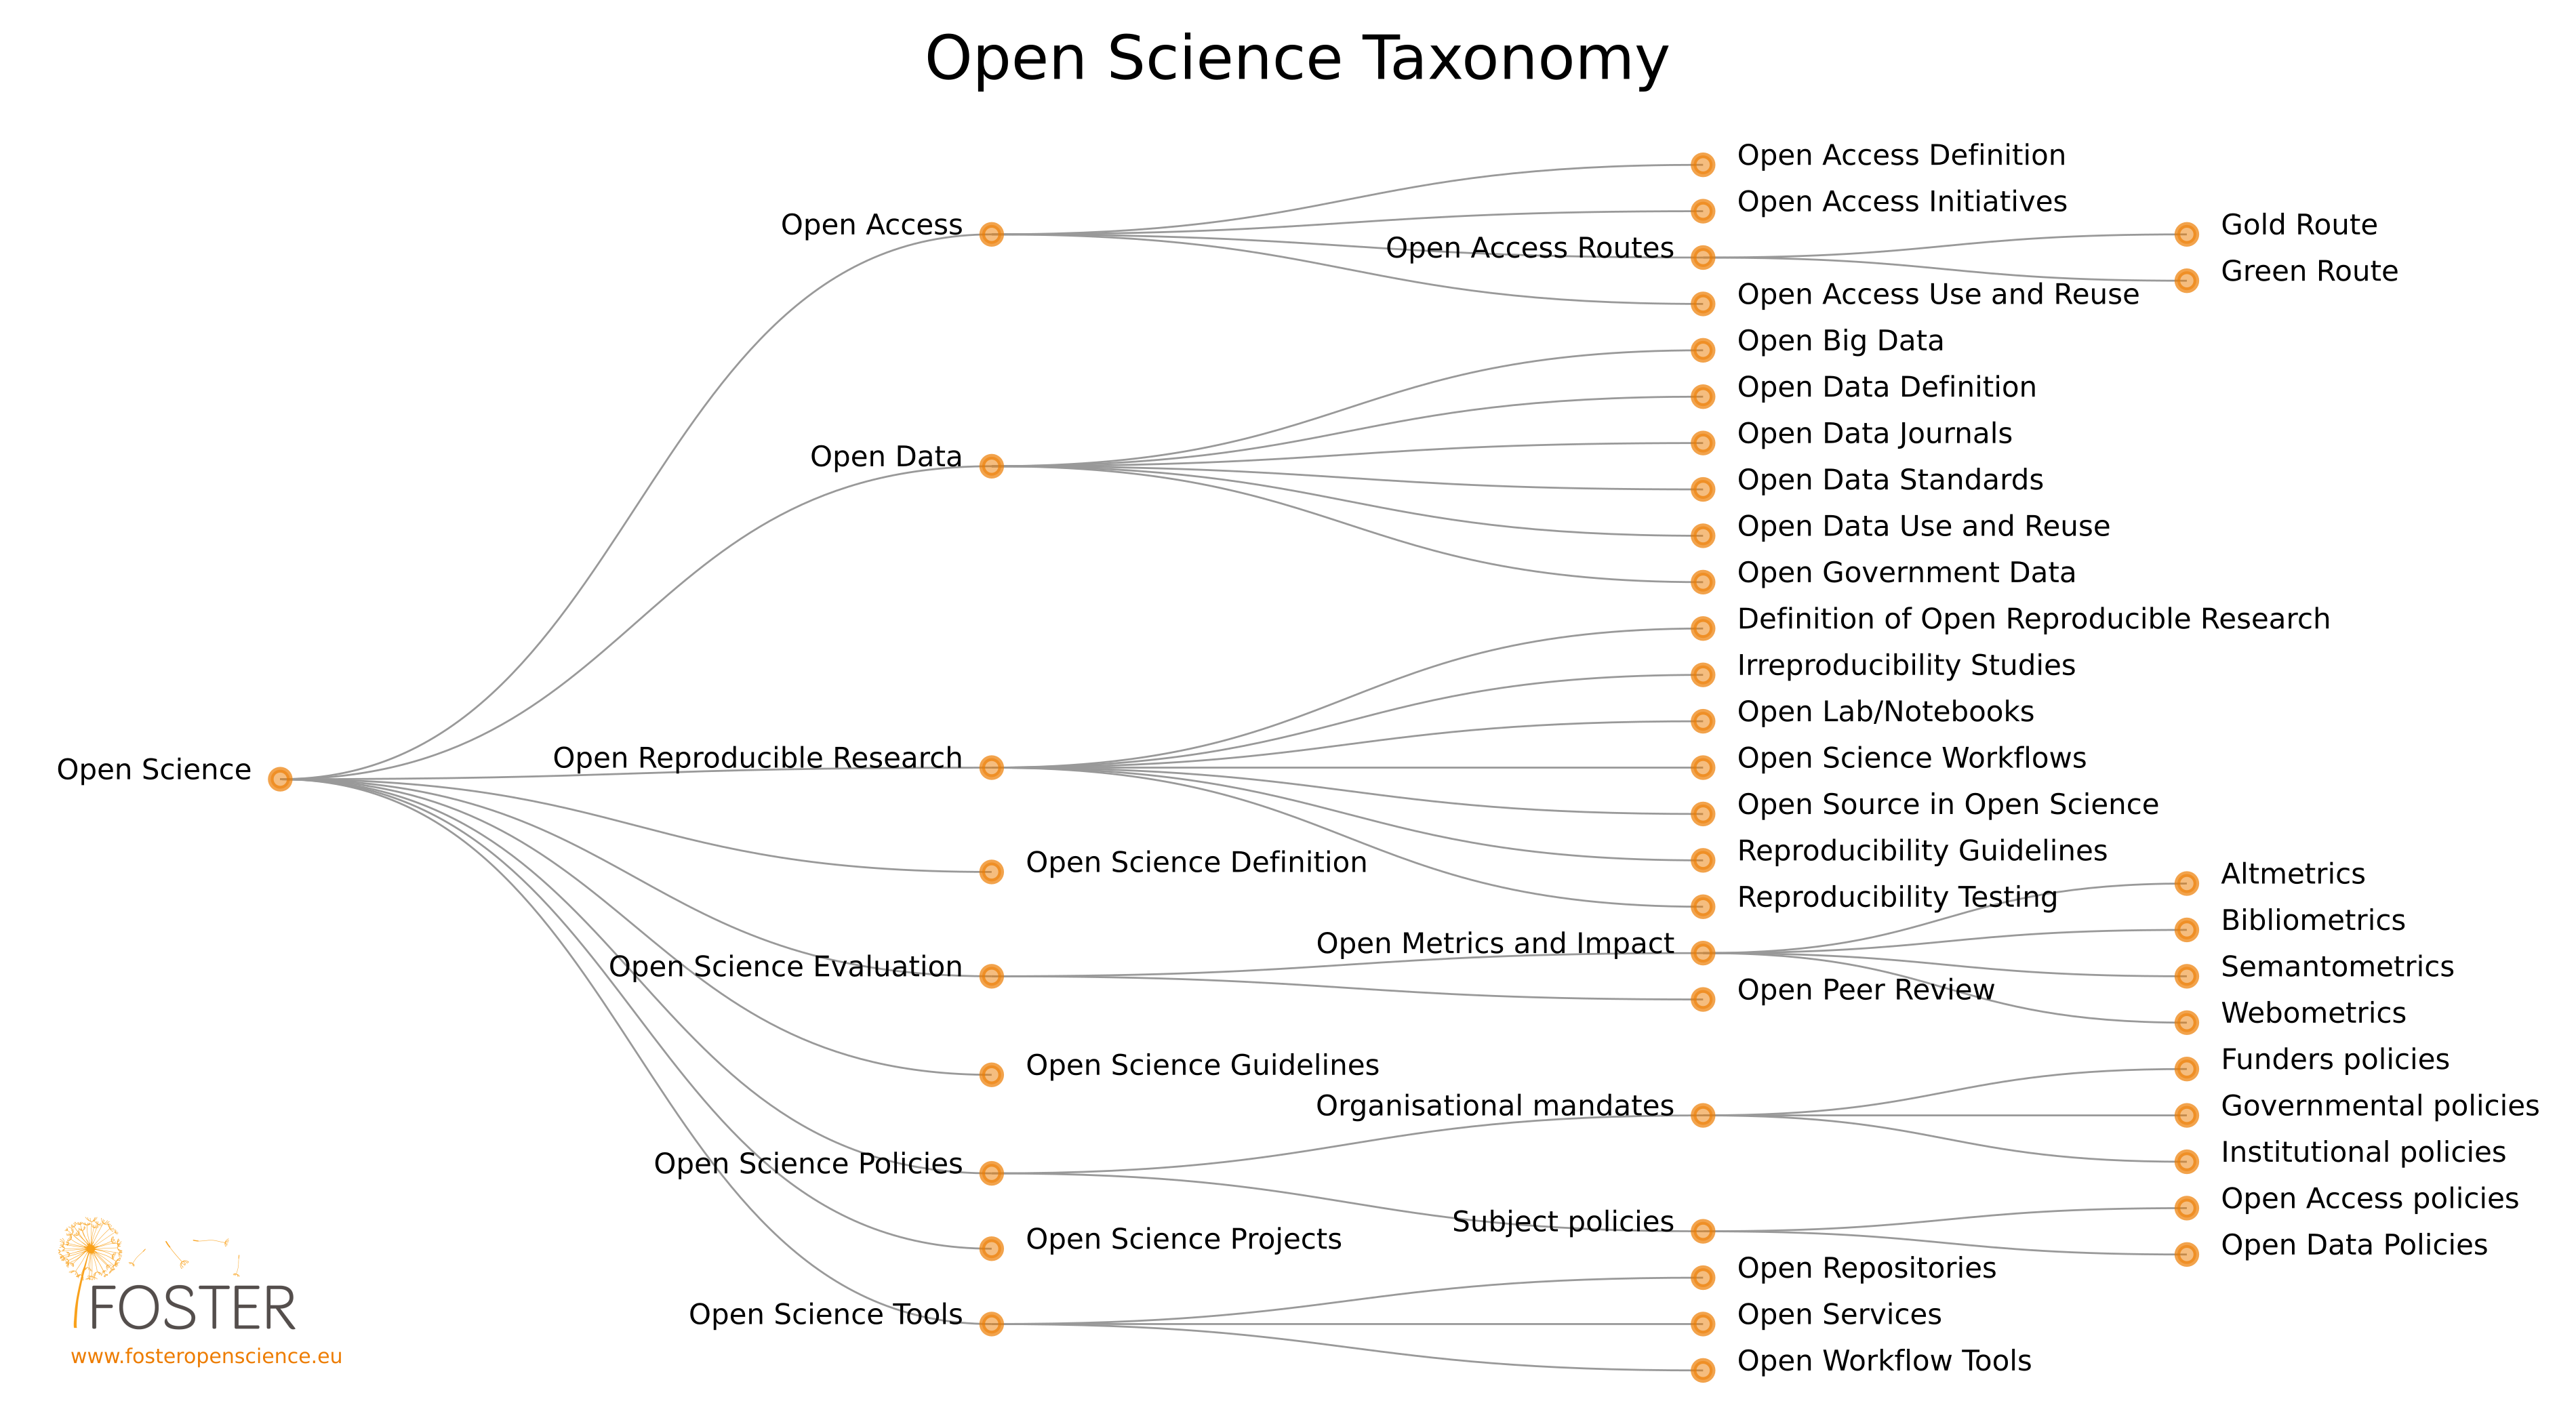
\includegraphics{images/os_taxonomy.png}
\caption{FOSTER Open Science taxonomy}
\end{figure}

FOSTER Open Science taxonomy

The different aspects of this will be explored throughout different modules in this MOOC, but here it is worth highlighting just some of the core concepts:

\begin{itemize}
\item
  \textbf{OPEN DATA}: Open data is the process of sharing both the original, raw and the treated or processed data online. This helps others to redo your experiments, and re-use it for additional purposes, helping to verify and accelerate research discoveries.
\item
  \textbf{OPEN ACCESS}: Allows anyone to access and re-use research published in journal articles without payment or restriction.
\item
  \textbf{OPEN PEER REVIEW}: This is a highly dimensional concept, including aspects to do with publishing review reports, revealing the identity of reviewers, and making peer review a more continuous and collaborative process.
\item
  \textbf{OPEN METHODS}: Where the process of the research has been documented in a sufficient detail to allow others to \emph{repeat}, \emph{reproduce}, or \emph{replicate} the work.
\item
  \textbf{OPEN SOURCE}: Much modern research relies on code and software, and Open Source is about providing free access and re-use rights to this to maximise its utility.
\end{itemize}

Other critical aspects of Open Science include \textbf{Public Engagement with Science}, \textbf{Open Educational Resources}, and \textbf{Open Advocacy} - all of which will be covered in later modules!

Modules covered throughout this MOOC

Another popular framing device is the `Open Science schools of thought', by \href{"</a></strong></p>

\begin{enumerate}
\def\labelenumi{\arabic{enumi}.}
\item
  The \textbf{Infrastructure school}, which is concerned with how the architecture of new technologies can help to make a more efficient research enterprise;
\item
  The \textbf{Public school}, regards the accessibility of knowledge creation to a wider audience;
\item
  The \textbf{Measurement school}, concerned with alternative methods of assessing scientific impact development;
\item
  The \textbf{Democratic school}, based around fundamental rights of access to knowledge; and
\item
  The \textbf{Pragmatic school}, concerning the role of collaborative research for more efficient knowledge creation and dissemination.
\end{enumerate}

Recently, the \href{https://zenodo.org/record/1323437\#.W2bIJSj7RPY}{Foundations for Open Scholarship Strategy Development} added a 6th to this, the \href{https://open-scholarship-strategy.github.io/site/\#Community}{Community and Inclusion school}, which is concerned with ensuring a diverse and inclusive community in the Open Scholarship space.

\hypertarget{how-open-science-impacts-you}{%
\section{How Open Science impacts you }\label{how-open-science-impacts-you}}

\href{Task_1.md}{\textbf{GO TO TASK 1: Defining how Open Science affects you}}

The most comprehensive overview of how Open Science impacts you comes from \href{https://elifesciences.org/articles/16800}{McKiernan et al. (2016)}, entitled `How open science helps researchers succeed.' There's not much point rewriting this, as it does such a good job of making a positive case based on a number of important dimensions already! Here's the abstract:

\begin{quote}
Open access, open data, open source and other open scholarship practices are growing in popularity and necessity. However, widespread adoption of these practices has not yet been achieved. One reason is that researchers are uncertain about how sharing their work will affect their careers. We review literature demonstrating that open research is associated with increases in citations, media attention, potential collaborators, job opportunities and funding opportunities. These findings are evidence that open research practices bring significant benefits to researchers relative to more traditional closed practices.
\end{quote}

The relative citation rate (OA: non-OA) in 19 fields of research. This rate is defined as the mean citation rate of OA articles divided by the mean citation rate of non-OA articles. Multiple points for the same discipline indicate different estimates from the same study, or estimates from several studies. (McKiernan et al., 2016)

\hypertarget{changes-in-research-evaluation}{%
\subsection{Changes in research evaluation }\label{changes-in-research-evaluation}}

The world of research evaluation is slowly changing. The way in researchers and their research is assessed governs virtually everything, as this defines the motivation and incentives behind certain behaviours. Typically, the venue of publication (i.e., the journal and its impact factor) have been considered to be of critical importance in research(er) assessment. However, in the last 5 years there has been a surge in uprising against this practice. As \href{http://occamstypewriter.org/scurry/2012/08/13/sick-of-impact-factors/}{Stephen Curry noted in 2012}:

\begin{quote}
So consider all that we know of impact factors and think on this: if you use impact factors you are statistically illiterate.
* If you include journal impact factors in the list of publications in your CV, you are statistically illiterate.
* If you are judging grant or promotion applications and find yourself scanning the applicant's publications, checking off the impact factors, you are statistically illiterate.
* If you publish a journal that trumpets its impact factor in adverts or emails, you are statistically illiterate. (If you trumpet that impact factor to three decimal places, there is little hope for you.)
* If you see someone else using impact factors and make no attempt at correction, you connive at statistical illiteracy.
\end{quote}

All hail the mighty impact factor! Illustration by John R. McKiernan, CC BY

While there is generally little empirical evidence, it is generally accepted that research evaluation is almost entirely contingent on getting research articles published in `high impact' journal venues. Strangely, very little empirical evidence exists to demonstrate that this view is actually embedded in practice.

For example, a recent study from \href{https://hcommons.org/deposits/item/hc:21015/}{Juan Pablo Alperin and colleagues} analysed the review, tenure, and promotion guidelines from across a wide range of North American research institutes. What they found was that about 48\% of research institutes mention metrics of some sort in these documents, with variations across different institute types.

One consequence of this, is that other elements of the research process, are often seen as less important. This includes Open Science, and forms of wider public engagement, which can be viewed as risky or detrimental to the career choices of an individual research; in particular those who are already disadvantaged/marginalised, or at an earlier stage in their career.

This makes total sense. Researchers, believe it or not, are human. Thus, they are driven by inherent human desires to do things like pay their rent, eat food, pay bills, and provide for their families. In order to do this, they have to keep their jobs. Usually, this means conforming to how they believe they will be assessed, and any external pressures to this are seen as a risk to their livelihoods. This is why, as we discussed above, presenting `Open Science' as divergent from traditional research processes, as opposed to being enhanced or more beneficial ways of doing things, can actually be inadvertently damaging.

Perhaps a much bigger consequence of this, however, is that we essentially have a system where researchers are rewarded for how many papers they publish, and the brands associated with the venue of publication, which can be detrimental to the value of shared knowledge. For example, research has shown that using journal rank for research assessment is an inherently bad scientific practice, and indeed such a negative impact on research that scholarly journals should be abandoned altogether \href{https://www.frontiersin.org/articles/10.3389/fnhum.2013.00291/full}{(Brembs et al., 2013)}. Further research has also shown that journal rank is associated with decreased methodological quality and research reliability, and that the present system of journal hierarchies is an ongoing threat to the entire research system \href{https://www.frontiersin.org/articles/10.3389/fnhum.2018.00037/full}{(Brembs, 2018)}.

These issues and criticisms have led to an increasing debate around, and action against, modern research evaluation systems. One of the most significant steps was the development of the \href{http://www.leidenmanifesto.org/}{Leiden Manifesto}, which produced 10 simple principles to improve the measurement of research performance. It is presently available in \href{http://www.leidenmanifesto.org/translations.html}{20 languages}.

Another important step in research evaluation reform is the San Francisco \href{https://sfdora.org/}{Declaration on Research Assessment}, often shortened to DORA. Similarly to the Leiden Manifesto, DORA seeks to improve how research is assessed, and individuals and organisations can sign the declaration to show their support.

\hypertarget{potential-impact-on-your-career}{%
\subsection{Potential impact on your career }\label{potential-impact-on-your-career}}

Things are changing, though. It is becoming more widely realised that these publication-based incentives are detrimental to the research process, and the health of research culture. For example, this comes from an \href{http://www.nicebread.de/open-science-hiring-practices/}{advertisement for a professorship at the Ludwig Maximillian University}, Munich, and is one of the first times that Open Science was made an explicit part of hiring criteria:

\begin{quote}
``Our department embraces the values of Open Science and strives for replicable and reproducible research. For this goal we support transparent research with open data, open material, and pre-registrations. Candidates are asked to describe in what way they already pursued and plan to pursue these goals.''
\end{quote}

Having Open Science as a core value in research departments sends a strong message for a shift in research cultures. More and more universities all the time are including aspects of open scholarship in their promotion and tenure guidelines, including \href{http://whyopenresearch.org/promotion}{Virginia Commonwealth University, the University of North Texas, Harvard School of Engineering and Applied Sciences, Purdue University Indianapolis, and more}.

Another thing that researchers like to have in order to carry out their work is funding. Again, open practices are becoming much more widely recognised in the funding application process, and can even help to give researchers an edge, or the ability to qualify for special funds. Such funders include the \href{http://whyopenresearch.org/funding}{Bill and Melinda Gates Foundation, the National Science Foundation (USA), the National Institutes of Health (USA), the European Commission, the Wellcome Trust, and the Shuttleworth Foundation}). (note that the latter partially supported the development of this MOOC!)

The Registry of Open Access Repository Mandates and Policies (ROARMAP) is a searchable international registry charting the growth of open access mandates and policies adopted by universities, research institutions and research funders that require or request their researchers to provide open access to their peer-reviewed research article output by depositing it in an open access repository.

\hypertarget{creating-your-digital-profile}{%
\subsection{Creating your digital profile }\label{creating-your-digital-profile}}

Alright, enough talk for now. Or text, anyway. Let's help you build your personal, digital persona that embraces openness! Thankfully, you don't have to start from scratch here, and some smart folks have done a lot of the groundwork for you.

There now exist a range of cool tools that can help you to document your `open' research practices, and build this in to your own digital researcher profile. Here are some of the most important ones, and then a nice practical task to help you set them up for yourself!

\begin{itemize}
\item
  \textbf{ORCID} - This stands for Open Researcher and Contributor ID. ORCID gives you a persistent identifier for you and your research, and is a breeze to integrate with your entire publication record.
\item
  \textbf{ImpactStory} - Here, imagine all of the attention your research has received online brought to you in one place, linked with your ORCID profile, and displayed with cool badges and summaries? ImpactStory cleverly does this, and tells you your, er, impact story!
\item
  \textbf{Publons} - Don't you just hate it when you do a peer review, and then pretty much no one knows anything about it? Don't you want credit for all your hard work? Publons gives you a place to do that!
\item
  \textbf{Open Science Framework} - An open source software project that facilitates open collaboration in science research. Currently also hosts a range of preprint servers.
\end{itemize}

OK, let's go to Task 2 and get you set up with these.

Before you start, please be aware that Publons recently got acquired by the for-profit company Clarivate Analytics recently. While such acquisitions are fairly commonplace in this ecosystem, we want to make you aware that if you sign up to this organisation, while it does provide a value to you, it also uses you as the product which it uses to sell services. We recognise that some of you might be uncomfortable with this (think Facebook for peer review), and therefore this stage is totally optional based on your own values here.

\href{Task_2.md}{\textbf{GO TO TASK 2: Developing your digital researcher profile}}

\hypertarget{barriers-and-limitations-for-open-science}{%
\section{Barriers and limitations for Open Science }\label{barriers-and-limitations-for-open-science}}

Despite the more or less obvious benefits of Open Science practice (as discussed above), there are a range of reasonable concerns and therefore necessary limitations and exceptions to be identified, discussed and implemented in a highly discipline-specific manner. It would be utterly foolish, and not very scientific, of us to rampantly support Open Science without paying due consideration to these.

Such concerns include and are not limited to:

\begin{itemize}
\item
  Release of personal data of and information about individuals;
\item
  Publishing of any sensitive information (for example, bioengineering and medical information);
\item
  Geomapping data of endangered species (flora \& fauna);
\item
  Poor formatting of data for re-use;
\item
  Lack of distributed article-processing charge funding;
\item
  Use of proprietary software;
\item
  Financial paywalls imposed by publishers;
\item
  Complex, confusing, and difficult to navigate embargo periods;
\item
  Conflicts between funder and publisher policies;
\item
  Usage restrictions imposed by publisher; and
\item
  Reluctance to publish due to fear of competition.
\end{itemize}

Another important aspect to note (as has always been) is that each openly released dataset requires a clear description of the context in which the data was raised (i.e., metadata), so that researchers who make use of the freely accessible data apply it in a meaningful analysis and reasonably transferred context. Many of these are discussed further within the \href{https://open-scholarship-strategy.github.io/site/\#Challenges}{Foundations for Open Scholarship Strategy Development}.

Open Science reflects the intentions of the researchers themselves, and is thereby subject to cultural bias. Open Science is not a perfect system by any means, and operates a hierarchy between different barriers. For example, Open Access seeks to remove barriers such as price for readers and re-use permissions, but often fails to address barriers such as connectivity or language, and also in cases erect new barriers, such as author-facing costs.

This is something which the Open Science movement is becoming more and more aware of, especially regarding the risks and impacts that progress towards Open Science can have, particularly on marginalised demographics or already higher-risk communities. Some of the major barriers towards Open Science include:

\begin{itemize}
\item
  Forcing junior researchers to share their data at point of first publication, potentially compromising their future research based on those data;
\item
  High article processing charges (APCs) for publication, that discriminate against those without financial privilege;
\item
  Other \href{https://medium.com/@denalbz/power-and-inequality-in-open-science-discourses-9d425b0c2b63}{geopolitical factors} include resistance to sharing due to fear of persecution, and knowledge misuse or appropriation;
\item
  Evidence. Researchers are generally conservative to adoption of new approaches, until there is sufficient evidence that they are superior than traditional methods.
\end{itemize}

However, as well as these, there are several worrying and ongoing trends that reflect more systemic issues within Open Science, and scholarship more generally:

\begin{itemize}
\item
  That Open Science is introducing more metrics to `incentivise' researchers to work harder, at the cost of true productivity and creativity, and not always in their best interests;
\item
  That new gate-keepers are consolidating these metrics, and using them to define the future of research, ending up with a system operating more like a business than an exploratory venture;
\item
  The increasing capture of research and infrastructure by commercial, for-profit entities, reflecting the increasing neoliberal market organisation around science and higher education;
\item
  These same entities often having a parasitic relationship with researchers, who provide labour, services, and content for free to help them build profits;
\item
  A lack of job stability or security and resources, which acts against innovation or any form of risk-taking;
\item
  A lack of consideration of the social and cultural real-world benefits of research; and
\item
  The fact that most historical research still remains locked away from access or re-use.
\end{itemize}

Based on this, it is interesting to ask why such dangerous trends seem to grow from seemingly good intentions based on positive core principles and values. It might be easy, based on the above, to become extremely pessimistic, or even antagonistic, towards Open Science. However, as with any movement or new way of doing things, it is down to each of us to carefully balance the potential drawbacks and benefits, and the wider consequences and contexts of these.

While the core principles underlying Open Science are often focussed around accessibility, in practice there is often a trade-off within this hierarchy, and often with unforeseen consequences. Much of this is not due to the intentions of Open Science, but more about the difficulties in reconciling the different stakeholder viewpoints, which often leads to inherent conflict and complications around developments.

It is perfectly natural for researchers and industries that have made themselves successful or profitable based on a particular set of practices to resist any disruption towards that. Let us take several primary examples for this.

\begin{enumerate}
\def\labelenumi{\arabic{enumi}.}
\tightlist
\item
  Moving research evaluation away from journal brands and the impact factor.
\end{enumerate}

Imagine if you are a researcher who has built a successful career, to some extent based on the journals in which you have published your work. Then imagine someone says that journal brands, impact factors, and journal ranks are actually bad for science, and don't tell us much about the quality of your research. There's a chance you're going to resist that a bit.

Now, imagine if you are a commercial publisher. Selling your brand to libraries, funders, research assessment groups, and researchers it critical for the financial sustainability and integrity of your journal. Simply removing all concept of brands for your, er, brands, is not exactly a path to fiscal sustainability.

\begin{quote}
``We also aim at increasing APCs by increasing the value we offer to authors through improving the impact factor and reputation of our existing journals.'' - Springer Nature IPO (\href{http://web.archive.org/web/20180507134223/http:/proxy.dbagproject.de/mediacenter/ressourcen/pdf/emissionen/springernature_prospectus.pdf}{page 99}).
\end{quote}

Does this sound like a company who has the best interests of researchers, the public, and open science at heart? So there are major tensions here, that reflect inherent power dynamics within the scholarly communication system. Which perhaps explains why it has been so difficult to move away from an impact factor or journal dominated system since the advent of Open Science. At least part of this can be explained by a largely \href{https://zenodo.org/record/1472045\#.W-7r8ZP7RPY}{dysfunctional scholarly publishing `market'}.

\begin{enumerate}
\def\labelenumi{\arabic{enumi}.}
\setcounter{enumi}{1}
\tightlist
\item
  Moving away from a subscription model to one where all information is freely available.
\end{enumerate}

Did you know that back in 2007, publishers such as Elsevier, Wiley, and the American Chemical Society were advised by the \href{https://www.nature.com/articles/445347a}{`pitbull of PR'} to equate public/open access with government censorship, and for traditional subscription-based publishing with peer review? This is just one small part of a long history where some in the scholarly publishing industry have lobbied and ran smear campaigns against open access, as a delay tactic until they could find a way to either destroy it, or convert it into a profitable business model. This resistance perhaps is one of the key factors in explaining why, in after about 20 years of relentless campaigning, we have only made about 25\% of the world's research openly accessible, with the rest locked behind expensive paywalls.

\hypertarget{open-science-and-reproducible-research}{%
\section{Open Science and reproducible research }\label{open-science-and-reproducible-research}}

There is an enormous overlap between Open Science and reproducible research. Now, traditionally, much of the research process, as well as the outputs, remain hidden or closed from public scrutiny. Open Science attempts to expose some of this process; for example, by recording and documenting `failed' reactions, highlighting repeated experiments and their variants, and revealing thoughts, ideas, and comments that were part of the process but wouldn't make into a final research paper.

It might help to imagine Open Science practices as having a magnifying glass or webcam pointing at your research all the time. This helps to `expose' the process, increase care, and lead to a well-documented process that others can copy and replicate if needed. This is an inherently social process, but comes with an important consideration:

\textbf{Research is not a perfect process.}

This might be difficult to accept for many of us, as typically the research we read about in papers or in the media is just the `positive' aspects, with all of the gritty bits hidden from public view. We all know that research is imperfect, and we should learn to embrace and communicate failure as an inherent part of that process.

All of these elements can be documented as part of a `lab notebook', and comes with an important implication: \textbf{The aspects of research that did not produce favourable results are just as important as those which do.}

Here, the intersection of reproducibility and Open Science becomes centred around one a core value we discussed before: \textbf{Freedom and Liberation}. As \href{"</a></strong></p>

\begin{enumerate}
\def\labelenumi{\arabic{enumi}.}
\item
  Enable transparent and comfortable exploration of data;
\item
  Reward quality, which is under our control, rather than outcomes, which are not;
\item
  Reduce the demand for ``positive'' results required for career advancement;
\item
  Cultivate a flexible and open mindset;
\item
  Enable a more constructive and collaborative research climate; and
\item
  Generates more accurate information that is ultimately more accessible.
\end{enumerate}

Therefore, one could easily argue that Open Science is aligned with concepts of \textbf{academic freedom}, by liberating individuals from the constraints of the closed system. We will explore the links between Open Science and reproducible research more in \href{https://wikituneleu/modules/reproducible-research-and-data-analysis/}{Module 3}.

\hypertarget{making-open-science-part-of-your-daily-research-workflow}{%
\section{Making Open Science part of your daily research workflow }\label{making-open-science-part-of-your-daily-research-workflow}}

As you might now see, Open Science impacts almost every aspect of your typical research workflow. We all think, we all gather data and analyse it, and we usually want to share the results of this with virtually anyone who will listen and re-use it. There are a number of tools, services, platforms, and practices for you to engage with, and this will likely differ for each individual, lab group, or community.

There are no set rules though. Open Science gives you the freedom to explore processes that work best for you, your research, and the impact that can have on your wider community. Below is just one combination of examples of tools that can make your research workflow more open all the way from an initial grant proposal through to research assessment.

\begin{figure}
\centering
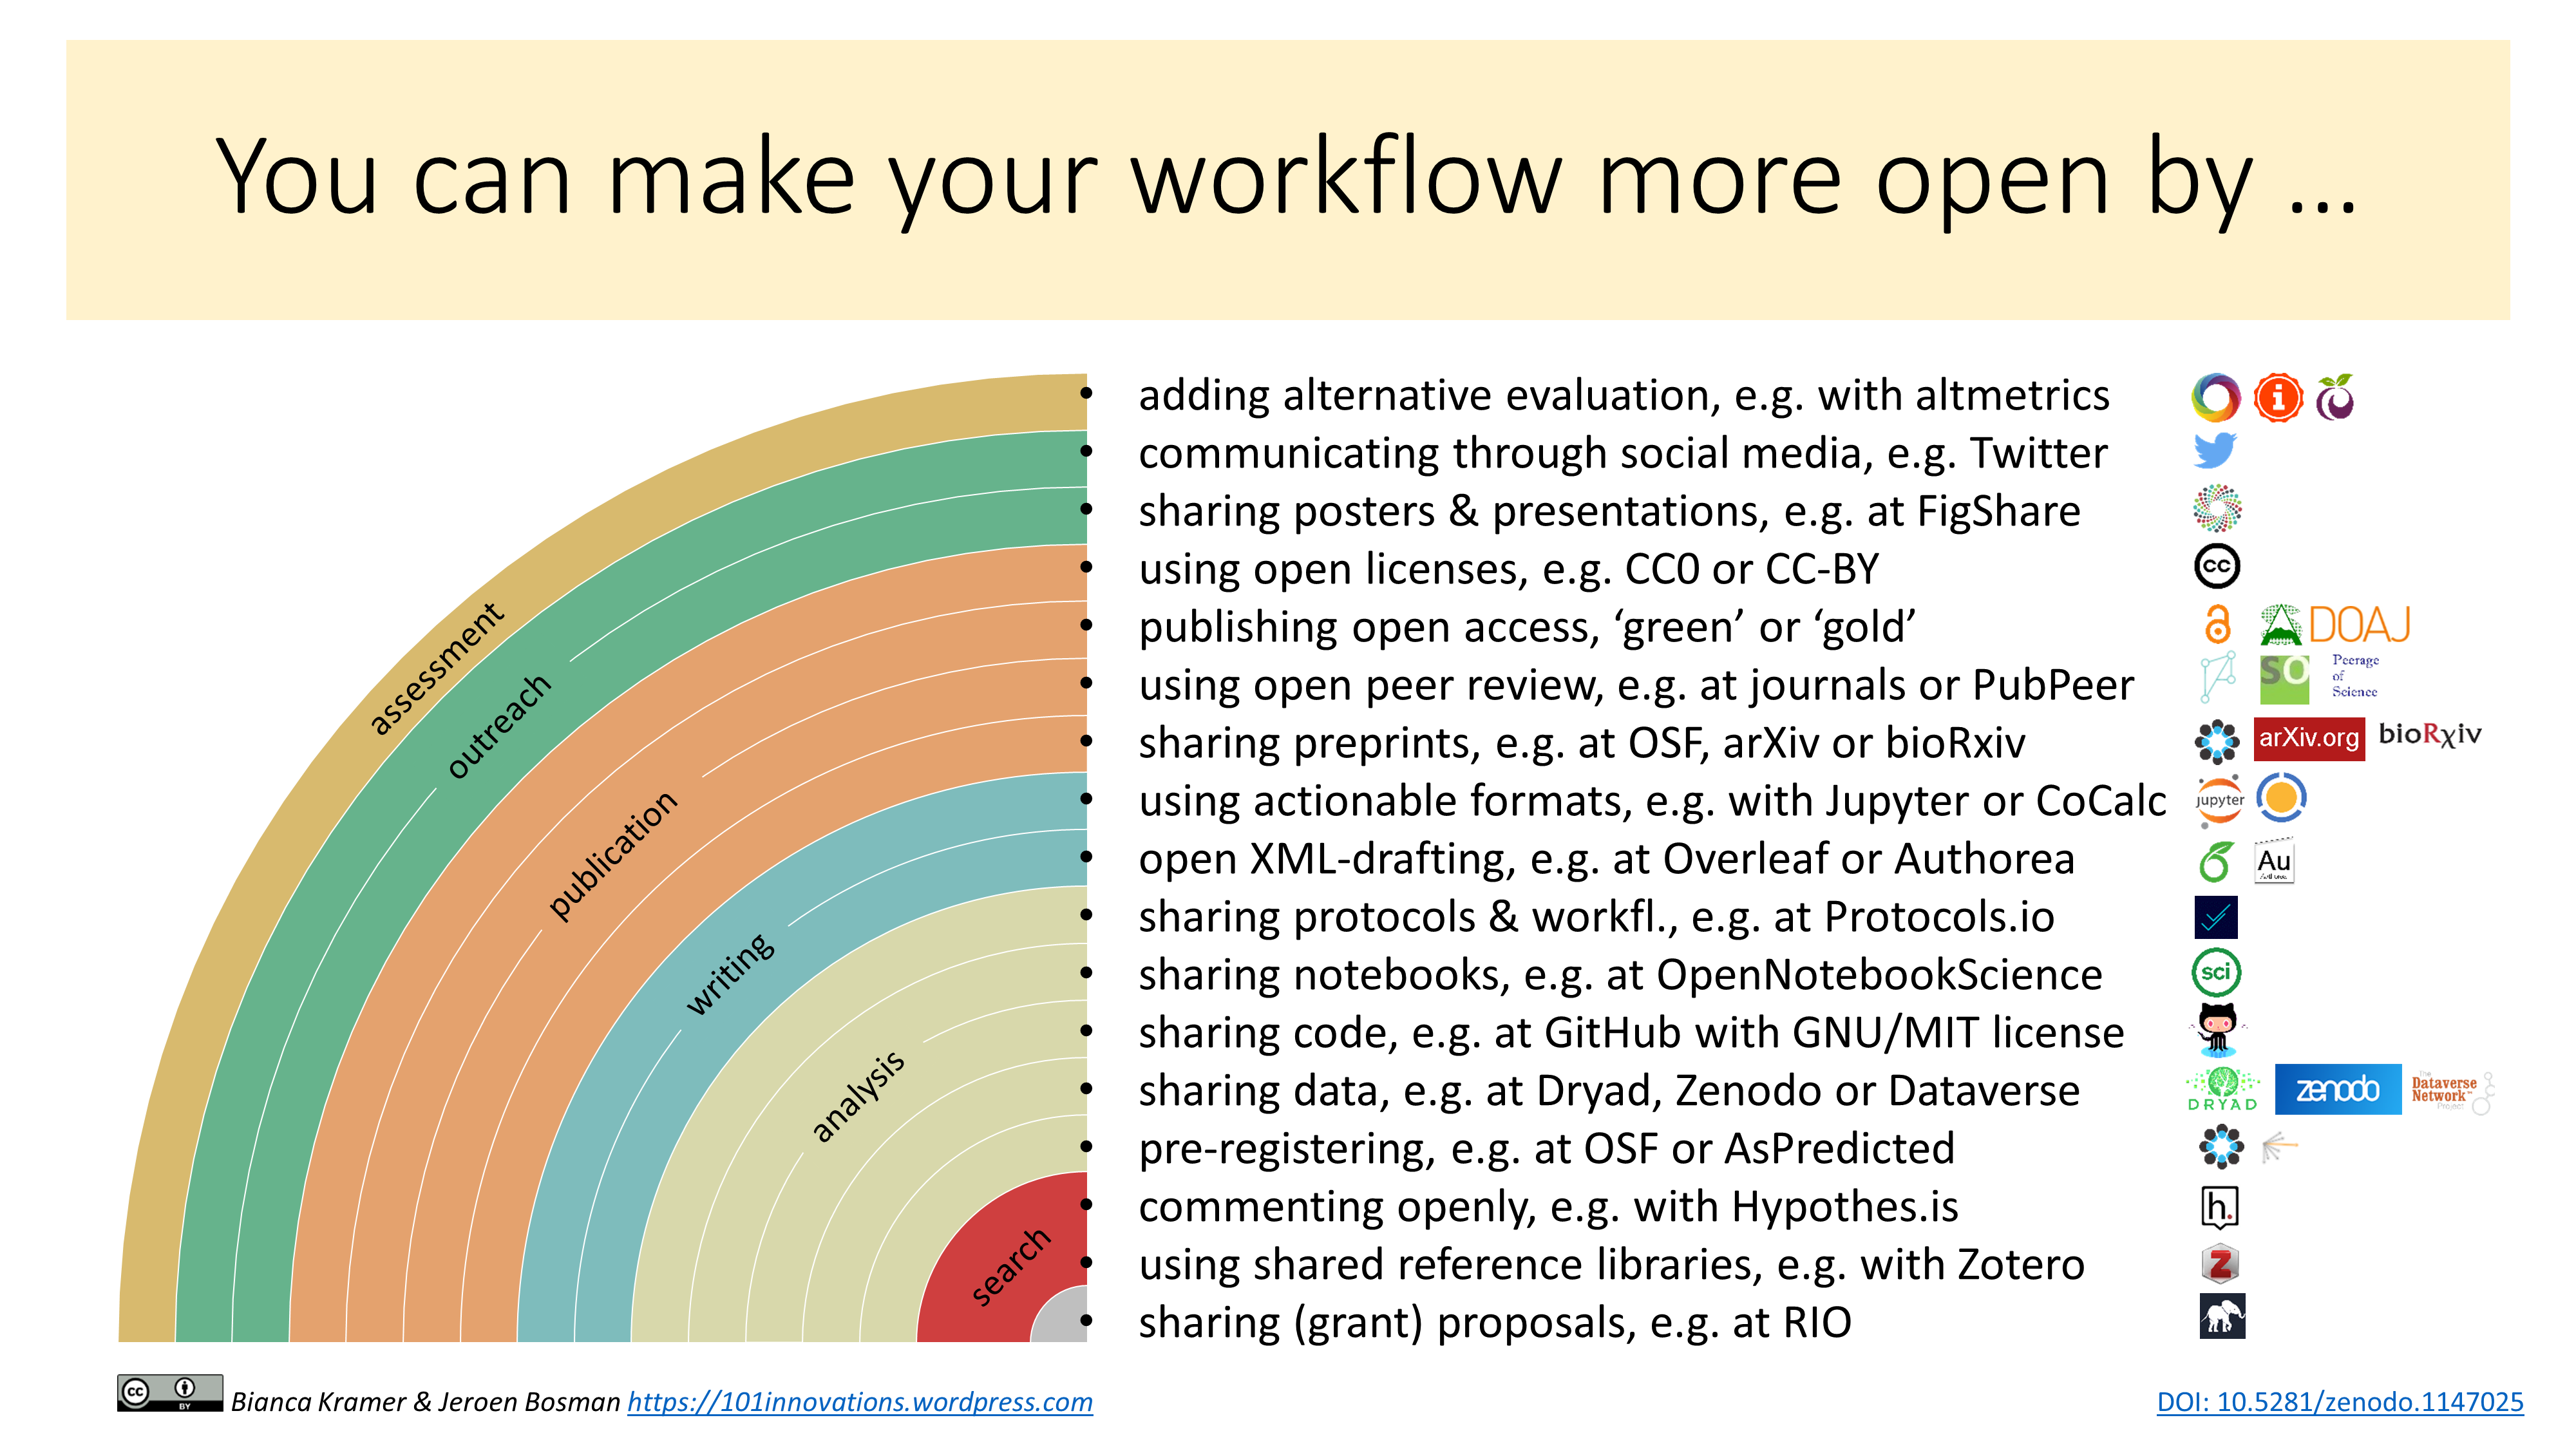
\includegraphics{images/rainbow-of-open-science-practices.png}
\caption{Rainbow of Open Science Practices}
\end{figure}

Kramer, Bianca, \& Bosman, Jeroen. (2018, January). Rainbow of Open Science practices. Zenodo. http://doi.org/10.5281/zenodo.1147025

Throughout the rest of this \href{https://wikituneleu/}{MOOC}, you will meet many of these on your Open Science adventure, and tailor new knowledge and skills to suit what is best for you.

\hypertarget{where-to-go-from-here}{%
\section{Where to go from here }\label{where-to-go-from-here}}

Hopefully now you have come to see the importance of Open Science as a fundamental part of modern research. Open Science is an umbrella term for a range of ideals, values, practices, and principles, all of which are integrated together:

\href{https://www.youtube.com/watch?v=Es7qvO_2kSg}{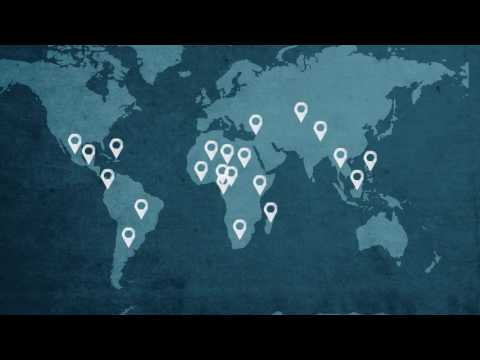
\includegraphics{images/0.jpg}}

Intersections of Openness: Open Access, Science, \& Education. By Abby Elder, CC BY 4.0 International License. Source

The \textbf{learning outcomes} from this for you should be:

\begin{itemize}
\item
  You will now be able to describe some of the ethical, social, cultural, and research impact arguments for and against Open Science.
\item
  After deciding which platforms/tools/services are most useful for yourself and your community, you will be able to develop a personal profile for showcasing their research profile and outputs.
\item
  After reflecting on the status of Open Science within your research group or lab, you will help to devise concrete ways to locally improve open practices.
\item
  Using the guidelines published by your research laboratories, departments, or institutes, you will be able to help identify the practices and policies for career progression and assessment, publishing and Open Access, and data sharing.
\item
  You will be able to further collaborate with colleagues and international peers to develop a shared definition of Open Science.
\end{itemize}

From these, what you will hopefully now have are the foundational best practices and knowledge needed to engage in Open Science. Some small, tangible steps you can take from here to make a real difference here include:

\begin{enumerate}
\def\labelenumi{\arabic{enumi}.}
\item
  Whenever possible, use and cite existing public data;
\item
  When you can, share your research data through a trusted online repository;
\item
  Make sure to release source code and scripts used for your analyses, including the environment needed to run them;
\item
  Post free copies of your research articles online however possible;
\item
  Share preprints of your research articles online, ideally at the time of journal submission; and
\item
  If you can, choose an Open Access journal to publish your research articles.
\end{enumerate}

These are adapted from \href{"</a></strong></p>

To learn more, visit the remaining 9 modules! This is the perfect chance for individuals, such as yourself, to take action and seize the initiative to become a champion in your research field.

\begin{quote}
Open Science is the future, and it will replace closed science. I encourage you to embrace it. - \href{("</a></strong></p>
\end{quote}

\hypertarget{further-reading}{%
\subsection{Further reading }\label{further-reading}}

There is so much potential material out there that it would take years of continuous reading to get through it all. Here are some favourite selected research articles on the topic that help to go into things a little deeper, and provide great overviews of much of what we have discussed here. All of them are free to access and re-use, of course!

\begin{itemize}
\item
  \href{"</a></strong></p>
\item
  \href{"</a></strong></p>
\item
  \href{"</a></strong></p>
\item
  \href{"</a></strong></p>
\item
  \href{"</a></strong></p>
\item
  \href{"</a></strong></p>
\item
  \href{"</a></strong></p>
\item
  \href{"</a></strong></p>
\item
  \href{"</a></strong></p>
\item
  \href{"</a></strong></p>
\item
  \href{"</a></strong></p>
\item
  \href{"</a></strong></p>
\item
  \href{"</a></strong></p>
\end{itemize}

\hypertarget{development-team}{%
\subsection{Development Team }\label{development-team}}

\begin{itemize}
\tightlist
\item
  \href{https://twitter.com/gtoneill}{Gareth O'Neill}, Language Lubber
\item
  \href{https://twitter.com/junanaguy}{Bruce Caron}, Culture Work Architect
\item
  \href{https://twitter.com/johave}{Jo Havemann}, \#ResearchinAfrica Highlighter
\item
  \href{https://twitter.com/protohedgehog}{Jon Tennant}, Dinosaur Whisperer.
\end{itemize}

\hypertarget{additional-tools-and-services}{%
\subsection{Additional tools and services}\label{additional-tools-and-services}}

\begin{itemize}
\item
  The \href{https://www.fosteropenscience.eu/toolkit}{FOSTER Open Science Training courses} are an excellent series for developing your Open Science skills. Each course takes about 1-2 hours to work through and you'll receive a badge upon completion. The courses include practical tips on getting started with Open Science as well as providing information on discipline specific tools and resources you can use.
\item
  The \href{http://jrost.org/}{Joint Roadmap for Open Science Tools}, a community working link together existing Open Science platforms and services into a unified infrastructure.
\item
  The \href{http://www.righttoresearch.org/resources/OpenResearchGlossary/index.shtml}{Open Research Glossary}, designed to help provide some insight into some of the language surrounding `Open Scholarship'.
\item
  The Berkeley Initiative for Transparency in Social Sciences (BITSS) have an excellent MOOC on \href{https://www.bitss.org/events/mooc-transparent-and-open-social-science/}{Transparent and Open Social Science}.
\item
  The \href{https://www.scienceopen.com/search\#collection/69988c7e-1855-4007-ba94-caa4c4638b1f}{Scholarly Communication} Super Collection at ScienceOpen contains more than 1000 research articles, thematically organised on the topic. Most of these are also Open Access.
\item
  \href{http://whyopenresearch.org/}{Why Open Research?} is a fantastic website by \href{https://twitter.com/emckiernan13}{Erin McKiernan}, providing illustrations and information that help to support a strong case for Open Research.
\item
  The \href{https://open-scholarship-strategy.github.io/site/}{Foundations for Open Scholarship Strategy Development}, a document that aims to agree on a broad, international strategy for the implementation of open scholarship that meets the needs of different national and regional communities but works globally.
\item
  \href{https://www.edx.org/course/open-science-sharing-your-research-with-the-world}{Open Science: Sharing Your Research with the World} - A MOOC hosted by TU Delft through edX.
\item
  This \href{http://www.markhooper.io/openscience/\#-1:0100000000}{incredible visualisation} of the Open Science landscape by Mark Hooper. Mark was also the one who designed the original logos for our MOOC!
\end{itemize}

\textbf{Know a way this content can be improved?}

Time to take your new GitHub skills for a test-run! All content development primarily happens \href{"</a></strong></p>

\hypertarget{module2}{%
\chapter{Open Collaboration}\label{module2}}

\hypertarget{in-construction}{%
\section{In construction}\label{in-construction}}

This module has not been built yet.

You want to help make this happen ? Feel free to join us! Anyone can help, from no experience to very expert users. This project is carried out mostly by volunteer work. If you would like to contribute, please join our slack channel \href{https://osmooc.herokuapp.com/}{Sign up for Slack Open Science MOOC} or join our \href{https://open-science-mooc-invite.herokuapp.com/}{GitHub project team}.

\hypertarget{module3}{%
\chapter{Reproducible research and data analysis}\label{module3}}

\hypertarget{in-construction-1}{%
\section{In construction}\label{in-construction-1}}

This module has not been built yet.

You want to help make this happen ? Feel free to join us! Anyone can help, from no experience to very expert users. This project is carried out mostly by volunteer work. If you would like to contribute, please join our slack channel \href{https://osmooc.herokuapp.com/}{Sign up for Slack Open Science MOOC} or join our \href{https://open-science-mooc-invite.herokuapp.com/}{GitHub project team}.

\hypertarget{module4}{%
\chapter{Open research data}\label{module4}}

\hypertarget{in-construction-2}{%
\section{In construction}\label{in-construction-2}}

This module has not been built yet.

You want to help make this happen ? Feel free to join us! Anyone can help, from no experience to very expert users. This project is carried out mostly by volunteer work. If you would like to contribute, please join our slack channel \href{https://osmooc.herokuapp.com/}{Sign up for Slack Open Science MOOC} or join our \href{https://open-science-mooc-invite.herokuapp.com/}{GitHub project team}.

\hypertarget{open-research-software-and-open-source}{%
\chapter{Open Research Software and Open Source}\label{open-research-software-and-open-source}}

\hypertarget{table-of-contents-1}{%
\section*{Table of Contents}\label{table-of-contents-1}}
\addcontentsline{toc}{section}{Table of Contents}

\begin{itemize}
\tightlist
\item
  \protect\hyperlink{Introduction}{Introduction}
\item
  \protect\hyperlink{What_OSS}{What is Open Source Software}
\item
  \protect\hyperlink{Principles}{Principles of Open Source Software}
\item
  \protect\hyperlink{OS_Community}{The Open Source community, governance, and contributions}
\item
  \protect\hyperlink{Platforms}{Existing platforms and tools for Open Source Software}
\item
  \protect\hyperlink{Research}{Open Source Software used in research}
\item
  \protect\hyperlink{FAQ}{Getting Started with OSS - FAQ}
\item
  \protect\hyperlink{Reuse}{Making good software for re-use}
\item
  \protect\hyperlink{Licensing}{Open Source licensing}
\item
  \protect\hyperlink{Citation}{Software citation}
\item
  \protect\hyperlink{GitHub_Zenodo}{Using GitHub and Zenodo}
\item
  \protect\hyperlink{Collaborating}{Collaborating through Open Source}
\item
  \protect\hyperlink{Future_OSS}{Where to go from here}
\end{itemize}

\textbf{PLEASE NOTE} that an audio version of this is available to download via \href{https://soundcloud.com/open-science-mooc/module-5-open-source-and-open-research-software}{Soundcloud} and \href{https://www.youtube.com/watch?v=BHrOEmKk5zM}{YouTube}.

\hypertarget{introduction-1}{%
\section{Introduction }\label{introduction-1}}

Welcome to \textbf{Module 5} of the Open Science MOOC: \textbf{Open Research Software and Open Source}.

This module has been developed \href{"</a></strong></p>

Don't forget you can join in the discussions over at our open \href{https://osmooc.herokuapp.com/}{\textbf{Slack channel}}. Please do introduce yourself at \#module5opensource, and tell us a bit about who you are, your background, and how you ended up here!

\hypertarget{who-is-this-module-for-1}{%
\subsection{Who is this module for?}\label{who-is-this-module-for-1}}

This module is designed primarily for computational researchers at the graduate and undergraduate level, as well as budding data scientists and any other researcher who uses analytical code or software. In a modern day research environment, this covers pretty much anyone who uses a computer for ther work.

\begin{quote}
``An article about computational result is advertising, not scholarship. The actual scholarship is the full software environment, code and data, that produced the result.'' - J. Buckheit and D. L. Donoho, 1995.
\end{quote}

Software and technology underpin much of modern research, which is now almost inevitably computational in one way or another - search engines, social networking platforms, analytical software, and digital publishing. With this, there is an ever-increasing demand for more sophisticated Open Source Software, matched by an increasing willingness for researchers to openly collaborate on new tools.

The power of Open Source is in that it lowers the barriers to collaboration and adoption, therefore allowing ideas and technology to spread more rapidly. This Module will introduce the necessary tools required for transforming software into something that can be openly accessed and re-used by others.

Image by Patrick Hochstenbach (CC0 1.0 Universal)

\hypertarget{specific-learning-objectives-for-this-module-1}{%
\subsection{\texorpdfstring{\textbf{Specific learning objectives for this Module}:}{Specific learning objectives for this Module:}}\label{specific-learning-objectives-for-this-module-1}}

\begin{enumerate}
\def\labelenumi{\arabic{enumi}.}
\item
  Learn the characteristics of open software; understand the \textbf{ethical, legal, economic, and research impact arguments for and against Open Source Software}, and further understand the quality requirements of open code.
\item
  Be able to turn code made for personal use into open code which is accessible by others.
\item
  Use software (tools) that utilizes open content and encourages wider collaboration.
\end{enumerate}

\hypertarget{what-is-open-source-software}{%
\section{What is Open Source Software }\label{what-is-open-source-software}}

Virtually all modern scientific research workflows rely on a range of software tools, either operating on different datasets, with different parameters, and applied iteratively in various ways (data science) or operating on different inputs and using models and methods to predict some output state (computational science). Open Source Software (OSS) is computer software in which the full source code is available under a specific license that enables other users to access, view, modify, and redistribute that code for any purpose. Because OSS requires such a license, it typically remains free of charge by default. This explicit licensing is also what differentiates OSS from free software. Re-using OSS for analysis, simulation and visualisation for research is also typically easier and more flexible compared to proprietary software. Often, whether we know it or not, we are already using OSS as part of our own research workflows.

OSS fits into the broader scheme of Open Science as it helps to make the full research environment, including the software that produced the research results, fully accessible and re-usable. As such, it forms a necessary component for the best practices (\href{"</a></strong></p>

In some cases, sharing of source code can even be conditional for the acceptance of associated research manuscripts (\href{"</a></strong></p>

Some of common advantages for developers include:

\begin{itemize}
\item
  Increased developer loyalty and empowerment;
\item
  Lower costs of services and marketing;
\item
  Increased branding of services and products;
\item
  Production of high quality software at lower expense;
\item
  Flexibility and rapid innovation;
\item
  Customisation and modular integration;
\item
  Increased reliability and independence; and
\item
  Based on open standards available to everyone.
\end{itemize}

As such, the main advantages for researchers (users) include \textbf{lower costs}, \textbf{increased transparency}, \textbf{increased security and stability}, \textbf{no vendor `lock in' with increased user control}, and \textbf{overall higher quality}. Furthermore, sharing OSS allows researchers to receive credit for their efforts, for example through direct software citation \href{"</a></strong></p>

Commonly used OSS include the \href{https://www.mozilla.org/en-US/firefox/}{Mozilla Firefox} internet browser and the \href{https://www.libreoffice.org/}{LibreOffice} full office suite. LibreOffice is similar to the popular Microsoft Office, including a word processor, spreadsheet manager, and slide presentation software, but is completely free and Open Source.

Some regard the OSS movement to represent a counter-movement to neoliberalism and privatisation, through defiance of regulations and norms in the construction and re-use of information, and a potential transformation of modern-day capitalism through making software abundantly available with minimal effort. See \href{http://www.redalyc.org/html/742/74212712006/}{The free/open source software movement: Resistance or change?} by Panayiota Georgopoulou for more on this topic.

\hypertarget{principles-of-open-source-software}{%
\section{Principles of Open Source Software }\label{principles-of-open-source-software}}

The \href{https://opensource.org/}{Open Source Initiative}, one of the pioneers of OSS, offers the following \href{https://en.wikipedia.org/wiki/The_Open_Source_Definition\#Definition}{definition}:

\emph{Don't worry, you don't need to memorise all of this, but it's good to know the principles that OSS is coming from.}

\begin{itemize}
\item
  \textbf{Free Redistribution}: The license shall not restrict any party from selling or giving away the software as a component of an aggregate software distribution containing programs from several different sources. The license shall not require a royalty or other fee for such sale.
\item
  \textbf{Source Code}: The program must include source code, and must allow distribution in source code as well as compiled form. Where some form of a product is not distributed with source code, there must be a well-publicized means of obtaining the source code for no more than a reasonable reproduction cost preferably, downloading via the Internet without charge. The source code must be the preferred form in which a programmer would modify the program. Deliberately obfuscated source code is not allowed. Intermediate forms such as the output of a preprocessor or translator are not allowed.
\item
  \textbf{Derived Works}: The license must allow modifications and derived works, and must allow them to be distributed under the same terms as the license of the original software.
\item
  \textbf{Integrity of The Author's Source Code}: The license may restrict source-code from being distributed in modified form only if the license allows the distribution of ``patch files'' with the source code for the purpose of modifying the program at build time. The license must explicitly permit distribution of software built from modified source code. The license may require derived works to carry a different name or version number from the original software.
\item
  \textbf{No Discrimination Against Persons or Groups}: The license must not discriminate against any person or group of persons.
\item
  \textbf{No Discrimination Against Fields of Endeavour}: The license must not restrict anyone from making use of the program in a specific field of endeavour. For example, it may not restrict the program from being used in a business, or from being used for genetic research.
\item
  \textbf{Distribution of License}: The rights attached to the program must apply to all to whom the program is redistributed without the need for execution of an additional license by those parties.
\item
  \textbf{License Must Not Be Specific to a Product}: The rights attached to the program must not depend on the program's being part of a particular software distribution. If the program is extracted from that distribution and used or distributed within the terms of the program's license, all parties to whom the program is redistributed should have the same rights as those that are granted in conjunction with the original software distribution.
\item
  \textbf{License Must Not Restrict Other Software}: The license must not place restrictions on other software that is distributed along with the licensed software. For example, the license must not insist that all other programs distributed on the same medium must be open-source software.
\item
  \textbf{License Must Be Technology-Neutral}: No provision of the license may be predicated on any individual technology or style of interface.
\end{itemize}

Now, this all might be a little complex to remember. However, it can be summarised as \emph{making software as re-usable as possible for future works, while also being freely available}.

\hypertarget{an-open-source-checklist}{%
\section{An Open Source checklist}\label{an-open-source-checklist}}

There are a number of existing platforms and tools that support OSS and collaboration. The \href{https://open-science-training-handbook.gitbook.io/book/}{Open Science Training Handbook} provides a check-list to use for evaluating the `openness' of existing research software, based on the Open Source Definition above:

\begin{itemize}
\item
  {[} {]} Is the software available to download and install?
\item
  {[} {]} Can the software easily be installed on different platforms?
\item
  {[} {]} Does the software have conditions on the use?
\item
  {[} {]} Is the source code available for inspection?
\item
  {[} {]} Is the full history of the source code available for inspection through a publicly available version history?
\item
  {[} {]} Are the dependencies of the software (hardware and software) described properly? Do these dependencies require only a reasonably minimal amount of effort to obtain and use?
\end{itemize}

Check, check, check, done! Simples.

\hypertarget{the-open-source-community-and-its-governance}{%
\section{The Open Source community and its governance }\label{the-open-source-community-and-its-governance}}

There are two main camps within the free software community: The \textbf{free software movement}, and the \textbf{OSS movement}. Both have differing ideologies based on user liberties and the practical applications of software. Often, the term `FLOSS' is used to reconcile these two political camps, and means `Free/Libre and Open Source Software'; Libre being French and Spanish for `free' in the context of freedom.

The core principle of re-use is what separates OSS from `Free Software'. Free and Open Source Software (FOSS) is an inclusive term to describe software that can be classified as both free and Open Source. A good example of FOSS is the \href{https://www.ubuntu.com/}{Ubuntu Linux} operation system.

The big difference between free software and OSS is that the former must distribute updated versions under the same license as the original, whereas newer versions of OSS can be distributed under different licenses. FOSS combines the best of both worlds.

These definitions have now become widely adopted, both by international governments, as well as some large organisations such as the \href{https://www.mozilla.org/en-US/foundation/}{Mozilla Foundation} and the \href{https://wikimediafoundation.org/wiki/Home}{Wikimedia Foundation}. Major organisations in the FLOSS space include the UK's \href{https://www.software.ac.uk/}{Software Sustainability Institute}, who produce valuable resources such as their recent \href{https://softwaresaved.github.io/software-deposit-guidance/}{Software Deposit Guidance for Researchers}.

\hypertarget{for-individual-projects}{%
\subsection{For individual projects}\label{for-individual-projects}}

A typical open source project has the following types of formal roles:

\begin{itemize}
\tightlist
\item
  \textbf{Author}: It is the person that created the project
\item
  \textbf{Owner}: The person/s who has administrative ownership over the organization or repository
\item
  \textbf{Maintainers}: Contributors who are responsible for driving the vision and managing the organizational aspects of the project. (They may also be authors or owners of the project.)
\item
  \textbf{Contributors}: The user that has already contributed to the project.
\item
  \textbf{Community Members}: People who use the project. They might be active in conversations, create new issues or express their opinion on the future project improvements.
\end{itemize}

Typically, roles are made public through either the \texttt{README} file, a Contributors file, or a separate team page for the project.

\hypertarget{existing-platforms-and-tools-for-open-source-software}{%
\section{Existing platforms and tools for Open Source Software }\label{existing-platforms-and-tools-for-open-source-software}}

Virtual environments and machines are becoming increasingly popular as high-powered research workflow enablers, and many of these are built upon OSS (e.g., operating systems, programming languages, and data processing frameworks). Popular services include \href{https://cloud.google.com/compute/}{Google Cloud} and \href{https://aws.amazon.com/}{Amazon Web Services}, which also assist with database storage and content delivery, as well as computational power. \href{https://insidedna.me/}{InsideDNA} is a computing platform for reproducible research in bioinformatics, genomics and the life sciences.

As mentioned \protect\hyperlink{What_OSS}{above}, LibreOffice provides an Open Source alternative to Microsoft Office. The two are almost completely compatible, just with different default file formats. For citation managers, \href{https://www.zotero.org/}{Zotero} is the most popular Open Source alternative to proprietary platforms such as Mendeley or EndNote.

\href{https://www.zotero.org/}{Zotero} uses the BibTeX (pronounced `bib-tech') format, based on LaTeX (pronounced `lay-tech'), and has browser plugins to make citation management simple. By integrating this with other software such as LibreOffice, it is now possible to have a fully Open Source research workflow in many cases.

\hypertarget{github}{%
\subsection{GitHub }\label{github}}

\begin{quote}
Did you know that this entire project was build as an open and collaborative community effort in \href{"</a></strong></p>
\end{quote}

\href{https://github.com/}{GitHub} is a popular hosting site for both software and non-software content (often called `notebooks'), with added capabilities for version control, project management and tracking, and storage services. GitHub is built on top of the OSS \href{https://git-scm.com/}{Git}, which enables users to work remotely to maintain, share, and collaborate on research software and other non-software based projects.

Version control is essentially a process that takes snapshots of the files in a repository, and tracks modifications to them. It records when the changes were made, what they were, and who did them. If several people are working on one file at once, any overlapping changes are detected, and must be resolved prior to continuing. This provides a much more streamlined and automated process than manually saving and recording changes as projects develop. It also avoids the inevitable lists of confusing named file versions\ldots{}

GitHub helps us to avoid, er, sub-optimal file naming conventions (source: XKCD)

One of the more popular and useful functions of GitHub is the \href{"</a></strong></p>

Other similar project hosting services include \href{https://bitbucket.org/}{BitBucket}, \href{https://about.gitlab.com/}{GitLab}, and \href{https://launchpad.net/}{Launchpad}. If the recent acquisition of GitHub by Microsoft is a bit off-putting to you, these are great alternatives.

However, we also know that GitHub can have quite a high learning curve. Which is why the first practical task for this MOOC will teach you how to set up your first GitHub project repository!

\textbf{\href{"</a></strong></p>

\hypertarget{open-source-software-used-in-research}{%
\section{Open Source Software used in research }\label{open-source-software-used-in-research}}

Especially in scientific research, Open Source Software usage and development has become practically the norm. There's a number of reasons for this beyond those that apply to the general acceptance of OSS by, for example, consumers, industry, or government. Among these reasons are:

\begin{itemize}
\item
  Increasingly, algorithms implemented in analysis software form an integral part of the methods described in scholarly publications. As such, it is completely at odds with rigorous peer review if these algorithm implementations are closed to outsiders.
\item
  Scientific collaboration more often than not spans multiple institutions and distributed research networks where secrecy and command hierarchy is not maintained in a way that is `necessary' for closed source development.
\item
  Many computational analyses are run in virtualized environments (such as institutional, national, or international `cloud' infrastructures) and hosted on multi-user servers. Closed-source, commercial software often disallows such usage.
\item
  OSS development often relies on volunteers. In a time of budgetary constraints for scientific research, this is a clear advantage.
\end{itemize}

For these and other reasons, Open Source tools are very commonly used in scientific research. This includes usage in fields where many researchers are amateur developers themselves and rely on tools such as \href{https://www.r-project.org/}{R} for statistical analysis and scripting, which, in the last decade, has almost completely displaced commercial software for statistical analysis such as SPSS or JMP in a lot of fields. In fields such as bioinformatics, that involve a lot of file handling of the outputs of DNA sequencing platforms, general purpose scripting languages such as \href{https://www.python.org/}{Python} and commonly used libraries built on top of it (such as \href{http://biopython.org}{biopython}) have become a vital part of the toolkit of many researchers.

Python

Tools such as R and Python are essentially software for writing software. Although programming is an increasingly common activity among researchers, of course not \emph{every} scientist does this. One step away from programming is the chaining together of the inputs and outputs of various analysis tools in longer workflows. As an example from genomics, a very common workflow is to start out with high-throughput sequencing reads and then i) do basic quality control checks; ii) map the reads against a reference genome; iii) identify the points where the new data are at variance with the reference. These steps are routinely executed as a workflow where a different Open Source executable is run in a Linux command-line environment for each of the three steps. Although this is arguably not quite open source software development, it does involve the usage and production of open source artifacts (such as Linux shell scripts) for which the principles that we discuss in this module are applicable.

R

Lastly, OSS is also used in scientific research for reasons that more closely mirror those that drive the adoption of OSS in wider society, namely that it is cheap. For example, individuals or organizations might decide to switch from Microsoft Office to LibreOffice for manuscript writing or spreadsheet processing because the latter is free (both as in \href{https://www.youtube.com/watch?v=dQw4w9WgXcQ}{\textbf{`free beer'}} and `free speech'). Likewise, the choice to switch from ArcGIS to \href{https://www.qgis.org/en/site/}{QGIS} for the analysis of geographic information might be prompted simply by cost considerations.

\hypertarget{getting-started-with-oss---faq}{%
\section{Getting Started with OSS - FAQ }\label{getting-started-with-oss---faq}}

\textbf{I'm using X{[}e.g.~Matlab,STATA,Excel{]} and I want to transition to something more open. What are the next steps?}

Even if you are using proprietary software, you can usually still share your source code/documents etc. \emph{The best first step is sharing whatever you can}.

\textbf{Great! I can put them in my new github repo.}

If that's enough for you for now great! If not for most pieces of proprietary software there are Open Source equivalents. Have a go with one and see what you think.

\begin{longtable}[]{@{}ll@{}}
\toprule
\begin{minipage}[b]{0.47\columnwidth}\raggedright
Closed\strut
\end{minipage} & \begin{minipage}[b]{0.47\columnwidth}\raggedright
Open\strut
\end{minipage}\tabularnewline
\midrule
\endhead
\begin{minipage}[t]{0.47\columnwidth}\raggedright
Matlab\strut
\end{minipage} & \begin{minipage}[t]{0.47\columnwidth}\raggedright
Python, Julia\strut
\end{minipage}\tabularnewline
\begin{minipage}[t]{0.47\columnwidth}\raggedright
STATA/SPSS\strut
\end{minipage} & \begin{minipage}[t]{0.47\columnwidth}\raggedright
R\strut
\end{minipage}\tabularnewline
\begin{minipage}[t]{0.47\columnwidth}\raggedright
MS Office\strut
\end{minipage} & \begin{minipage}[t]{0.47\columnwidth}\raggedright
LibreOffice\strut
\end{minipage}\tabularnewline
\begin{minipage}[t]{0.47\columnwidth}\raggedright
Mathematica\strut
\end{minipage} & \begin{minipage}[t]{0.47\columnwidth}\raggedright
JupyterLab\strut
\end{minipage}\tabularnewline
\begin{minipage}[t]{0.47\columnwidth}\raggedright
Test out your new \href{https://help.github.com/articles/about-pull-requests/}{Pull Request -PR-} Skills \ldots{}\strut
\end{minipage} & \begin{minipage}[t]{0.47\columnwidth}\raggedright
\ldots{} by adding your own example \href{"</a></strong></p>
\end{minipage}\tabularnewline
\bottomrule
\end{longtable}

\textbf{Cool! But if I make the switch will I be stuck: taking ages to learn a new tool/ without support /with buggy software.}

Good question! The answer is it depends. The best thing to do is find someone who's made the switch before and learn from their experience. Or just do a Google search! Some OSS is much better than their closed counterparts, some aren't, so it's worth choosing carefully.

\hypertarget{making-good-software-for-re-use}{%
\section{Making good software for re-use }\label{making-good-software-for-re-use}}

The most likely person who might want to re-use your software in the future is\ldots{}you! So while sharing is always better than not sharing, you can make your own life, and that of others, much easier through appropriate documentation. Documentation can include several things, such as including helpful comments and annotations in the code that help to explain why a particular action was performed, rather than what it is intended to achieve.

One of the most critical aspects of this is including an informative \texttt{README} file, that accompanies almost every OSS project, and some times even more than one. It can be a good practice to include one such file in every directory, that includes a list of files, a table of contents, and what the purpose of the directory is. The \texttt{README} file is typically just plain text or markdown (again, such as all of the ones for the MOOC!), and can include critical information for how to install and run software, previous dependencies and requirements, as well as tutorials or examples.

\begin{quote}
\textbf{Did you know\ldots{}} The term \texttt{README} is some times playfully ascribed to the famous scene in Lewis Carroll's Alice's Adventures In Wonderland in which Alice confronts magic munchies labeled with ``Eat Me''" and ``Drink Me''. Potent.
\end{quote}

The purpose here is to provide sufficient information to maximise the re-use and reproducibility of the computational environment, such that someone with no experience with the project can easily access and re-use the software (\href{"</a></strong></p>

An extension of this that can help to make things even easier for future re-use is `container' technology. Containers are like an ecosystem frozen in time, where the code, the data, any other dependencies, are all perfectly preserved, packaged and saved in the present functioning versions. This means that anyone in the future any one can come in and run the analyses again. As such, they are generally good for re-use, but this can come at the sacrifice of modification or understanding by others, as often a lot of details can be hidden within the source code and its dependencies. Common examples of container implementation in research include \href{"</a></strong></p>

\textbf{Sustainable software is good software.}

\hypertarget{simple-rules-for-reproducible-computational-research}{%
\section{10 simple rules for reproducible computational research}\label{simple-rules-for-reproducible-computational-research}}

The 10 simple rules for making computational research more reproducible, based on \href{"</a></strong></p>

\begin{enumerate}
\def\labelenumi{\arabic{enumi}.}
\tightlist
\item
  For every result, keep track of how it was produced.
\item
  Avoid manual data manipulation steps.
\item
  Archive the exact versions of all external programs used.
\item
  Version control all custom scripts.
\item
  Record all intermediate results, when possible in standardised formats.
\item
  For analyses that include randomness, note underlying random seeds.
\item
  Always store raw data behind plots.
\item
  Generate hierarchical analysis output, allowing layers of increasing detail to be inspected.
\item
  Connect textual statements to underlying results.
\item
  Provide public access to scripts, runs, and results.
\end{enumerate}

Infographic adapted from Sandve et al., (2013). Feel free to download this and print it out to keep handy during your research!

If you follow these steps, along with the processes in \href{"</a></strong></p>

\hypertarget{open-source-licensing}{%
\section{Open Source licensing }\label{open-source-licensing}}

An Open Source license is a type of license designed specifically for software and code that make it explicit what the legal conditions for sharing and re-use are. As mentioned \protect\hyperlink{What_OSS}{above}, the addition of a suitable license is what differentiates publicly shared software from OSS. For example, the widely used \href{https://www.mathworks.com/products/matlab.html}{MATLAB} is proprietary software, and \href{https://www.gnu.org/software/octave/}{Octave} is an openly licensed alternative programming language.

There are currently more than 1,400 unique Open Source licenses, a complexity born from the difficulty in understanding the differences between the legal implications across different license.

Some of the more common licenses include:

\begin{itemize}
\tightlist
\item
  \href{https://en.wikipedia.org/wiki/BSD_licenses}{Berkeley Software Distribution (``BSD'')},
\item
  \href{https://www.apache.org/licenses/LICENSE-2.0}{Apache},
\item
  \href{https://opensource.org/licenses/MIT}{MIT-style (Massachusetts Institute of Technology)}, or
\item
  \href{https://www.gnu.org/licenses/gpl-3.0.en.html}{GNU General Public License (``GPL'')}.
\end{itemize}

You don't need to know all the legal itty gritty behind all of these, but it is good to at least know what options are avaiilable to you.

There are two ways in which contributions to a project become licensed:

\begin{enumerate}
\def\labelenumi{\arabic{enumi}.}
\tightlist
\item
  \emph{Explicitly}, whereby the individual contribution has a clearly indicated license independent of the main project; or
\item
  \emph{Implicitly}, whereby the contribution falls under the original licensing code of the main project.
\end{enumerate}

Thankfully, the process of selecting an Open Source license is relatively trivial, thanks to user-friendly tools such as \href{https://choosealicense.com/}{Choose A License}. Each of these licenses allows other users to use, copy, distribute, and build upon your work, often while ensuring that the creators are appropriately recognised for their work. Here, the key is selecting an appropriate license for your work, depending on what you want, or do not want, others to do with it.

\hypertarget{software-citation}{%
\section{Software citation }\label{software-citation}}

Citations provide one of the most important interactions in scholarly research, forming the basis of our referencing and metrics systems. Typically, this is performed thanks to the assistance of a permanent unique identifier such as a \href{https://en.wikipedia.org/wiki/Digital_object_identifier}{Digital Object Identifiers} (DOI). A DOI is a persistent identifier, implemented in the \href{https://en.wikipedia.org/wiki/Handle_System}{Handle System}, that meets a common standard, depending on the purpose, such as for identifying academic information. Such identification is critical for tracking the genealogy and provenance of research, for reproducibility, as well as for giving appropriate credit to those who have created the software. Importantly, software should be considered a legitimate output from scholarly research, and citation is becoming an increasingly common way to indicate that.

In 2016, \href{"</a></strong></p>

\begin{itemize}
\tightlist
\item
  The author name(s),
\item
  Software title,
\item
  Version number, and
\item
  The unique identifier/locator (DOI or URL).
\end{itemize}

The six principles of software citation by \href{"</a></strong></p>

\begin{itemize}
\item
  \textbf{Importance}: Software should be considered a legitimate and citable product of research. Software citations should be accorded the same importance in the scholarly record as citations of other research products, such as publications and data; they should be included in the metadata of the citing work, for example in the reference list of a journal article, and should not be omitted or separated. Software should be cited on the same basis as any other research product such as a paper or a book, that is, authors should cite the appropriate set of software products just as they cite the appropriate set of papers.
\item
  \textbf{Credit and attribution}: Software citations should facilitate giving scholarly credit and normative, legal attribution to all contributors to the software, recognizing that a single style or mechanism of attribution may not be applicable to all software.
\item
  \textbf{Unique identification}: A software citation should include a method for identification that is machine actionable, globally unique, interoperable, and recognized by at least a community of the corresponding domain experts, and preferably by general public researchers.
\item
  \textbf{Persistence}: Unique identifiers and metadata describing the software and its disposition should persist - even beyond the lifespan of the software they describe.
\item
  \textbf{Accessibility}: Software citations should facilitate access to the software itself and to its associated metadata, documentation, data, and other materials necessary for both humans and machines to make informed use of the referenced software.
\item
  \textbf{Specificity}: Software citations should facilitate identification of, and access to, the specific version of software that was used. Software identification should be as specific as necessary, such as using version numbers, revision numbers, or variants such as platforms.
\end{itemize}

Note: For instructions on `how to make your software citable' see the section \protect\hyperlink{GitHub_Zenodo}{\textbf{Using GitHub and Zenodo}} below and \href{"</a></strong></p>

\hypertarget{using-github-and-zenodo}{%
\section{Using GitHub and Zenodo }\label{using-github-and-zenodo}}

\protect\hyperlink{GitHub}{GitHub} is a popular tool for project management, content storage, and version control. Note that GitHub itself is not OSS. However, Git, the tool which it is based on, is. Git is designed to help manage the source code files, and the updates to them, for a software-related project. However, it can also be extended to other non-software projects; for example, this \href{"</a></strong></p>

However, getting research onto GitHub is just the first step. It is equally important to make it persistent and re-usable, which is why having a Digital Object Identifier (DOI) associated with it can be useful. The simplest way to do this is through a service called \href{https://zenodo.org/}{Zenodo}, which is a free and open source multi-disciplinary repository created by OpenAIRE and CERN, and can be used to assign a DOI to individual GitHub repositories. There is a \href{https://guides.github.com/activities/citable-code/}{GitHub Guide} that explains the details, which involve linking GitHub repositories directly through to Zenodo so that when developers create formal releases for their software, Zenodo creates and archives a that version of the software.

There's nothing special about using Zenodo for creating DOIs, other than its \textbf{free of cost}; other general repositories can also be used, such as \href{https://doi.datacite.org/}{DataCite DOI Fabrica}, or your own institutional repositories such as \href{https://www.library.caltech.edu/news/enhanced-software-preservation-now-available-caltechdata}{Caltech's}.

A lot of researchers might typically be afraid of sharing code which is incomplete, buggy, or imperfect. However, in the OSS community, such a practice of sharing `raw' code is fairly commonplace. Sharing code openly enables others to re-use and improve it, as well as to engage in a deeper way with any research associated with it. This is one of the fundamental aspects of peer-collaboration, perhaps best exemplified by the traditional process of research manuscript peer review.

Task 2 will guide you through the process of linking a GitHub repository to Zenodo for archiving.

\begin{quote}
\textbf{Did you know\ldots{}} All content produced for this MOOC is available as part of a community in \href{https://zenodo.org/communities/open-science-mooc/}{Zenodo}?
\end{quote}

\textbf{\href{"</a></strong></p>

\hypertarget{collaborating-and-contributing-through-open-source}{%
\section{Collaborating and contributing through Open Source }\label{collaborating-and-contributing-through-open-source}}

Often, OSS is developed in a public, decentralised, collaborative manner between multiple contributors. The purpose of this is to enhance the diversity and scope of a project and its design, in order to become more beneficial and sustainable. Such an approach was famously likened to a `bazaar' model by Eric Raymond, an early OSS proponent. One of the major guiding principles of this is that of \textbf{peer production}, which relies on self-organised communities to regulate the development of content, co-ordinated towards a shared goal or outcome.

OSS projects rely heavily on volunteer collaboration, which often entails a constant flux of newcomers in order to become productive and sustainable (\href{"</a></strong></p>

\hypertarget{where-to-go-from-here-1}{%
\section{Where to go from here }\label{where-to-go-from-here-1}}

Hopefully now you have come to see the importance of software as a cornerstone of modern science, and the importance that OSS plays in this.

The \textbf{learning outcomes} from this should be:

\begin{enumerate}
\def\labelenumi{\arabic{enumi}.}
\item
  You will now be able to define the characteristics of OSS, and some of the ethical, legal, economic and research impact arguments for and against it.
\item
  Based on community standards, you will now be able to describe the quality requirements of sharing and re-using open code.
\item
  You will now be able to use a range of research tools that utilise OSS.
\item
  You will now be able to transform code designed for their personal use into code that is accessible and re-usable by others.
\item
  Software developers will be able to make their software citable, and software users will know how to cite the software they use.
\end{enumerate}

\textbf{BONUS TASK}

If you have completed \href{"</a></strong></p>

However, your Open Source journey does not stop here! This was just the beginning, and there are some incredible resources out there if you would like to do or learn more:

\begin{itemize}
\item
  If you feel particularly inspired by this, you can endorse the \href{http://sciencecodemanifesto.org/}{Science Code Manifesto}, which is based on the five principles of code, copyright, citation, credit, and curation.
\item
  To launch and develop your own project, the \href{https://opensource.guide/}{Open Source Guides} program offers a range of practical guides and skills to help launch and advance your OSS projects.
\item
  For a detailed look at OSS-based research workflows, the \href{https://pfern.github.io/OSODOS/gitbook/}{Open Science, Open Data, Open Source} hand-guide by Pedro L. Fernandes and Rutger A. Vos is one of the top resources online.
\item
  More formalised journal venues also exist for software-based articles, including \href{https://openresearchsoftware.metajnl.com/}{The Journal of Open Research Software} and \href{https://joss.theoj.org/}{The Journal of Open Source Software}. A list of such venues is also \href{https://www.software.ac.uk/which-journals-should-i-publish-my-software}{available}.
\item
  The \href{https://channels.plos.org/open-source-toolkit}{PLOS Open Source Toolkit} provides a global forum for Open Source hardware and software research and applications.
\item
  The \href{http://www.numfocus.org}{NumFOCUS} is a nonprofit organization that supports and promotes world-class, innovative, open source scientific software. Some of the projects they sponsor include:

  \begin{itemize}
  \item
    \href{http://ipython.org}{IPython} and \href{https://jupyter.org}{Jupyter Notebook} initiatives.
  \item
    \href{http://ropensci.org}{rOpenSci}, which promotes the open source R statistical environment for transparent and reproducible research.
  \item
    To gain more hands on experience with OSS, the \href{https://software-carpentry.org/}{Software Carpentry} community holds regular workshops to improve lab-based computing skills (\href{"</a></strong></p>
  \end{itemize}
\end{itemize}

\hypertarget{further-reading-1}{%
\subsection{Further reading }\label{further-reading-1}}

\emph{These references here are just the beginning. They include some of the most useful general overviews of the Open Source landscape in research. However, if you want to be find something more specific to your own research field, then that path is there for you to explore!}

\begin{itemize}
\item
  The Future of Research in Free/Open Source Software Development \href{"</a></strong></p>
\item
  The Scientific Method in Practice: Reproducibility in the Computational Sciences \href{"</a></strong></p>
\item
  The case for open computer programs \href{"</a></strong></p>
\item
  Current issues and research trends on open-source software communities \href{"</a></strong></p>
\item
  Ten simple rules for reproducible computational research \href{"</a></strong></p>
\item
  A systematic literature review on the barriers faced by newcomers to open source software projects \href{"</a></strong></p>
\item
  Knowledge sharing in open source software communities: motivations and management \href{"</a></strong></p>
\item
  Software citation principles \href{"</a></strong></p>
\item
  An introduction to Rocker: Docker containers for R \href{"</a></strong></p>
\item
  Good enough practices in scientific computing \href{"</a></strong></p>
\item
  Four simple recommendations to encourage best practices in research software \href{"</a></strong></p>
\end{itemize}

\hypertarget{development-team-1}{%
\subsection{Development Team }\label{development-team-1}}

\begin{itemize}
\tightlist
\item
  \href{https://twitter.com/alex__morley}{Alex Morley}, Open Sourceror, University of Oxford, UK.
\item
  \href{https://twitter.com/KMMoerman}{Kevin Moerman}, Open Sourceror, MIT, USA.
\item
  \href{https://twitter.com/ixek}{Tania Allard}, Open Sourceress, Data Enchantress, University of Leeds, UK.
\item
  \href{https://twitter.com/mrchristian99}{Simon Worthington}, Book Liberationist, TIB, Germany.
\item
  \href{https://twitter.com/pcmasuzzo}{Paola Masuzzo}, Open Source Batman, Italy.
\item
  \href{https://twitter.com/OAforClimate}{Ivo Grigorov}, Open Source Robin, Denmark.
\item
  \href{https://twitter.com/rvosa}{Rutger Vos}, Open Sourceror, Naturalis Biodiversity Center, the Netherlands.
\item
  \href{https://twitter.com/j_colomb}{Julien Colomb}, Open Ninja, Berlin.
\item
  \href{https://twitter.com/protohedgehog}{Jon Tennant}, Dinosaur Whisperer.
\end{itemize}

\textbf{Know a way this content can be improved?}

Time to take your new GitHub skills for a test-run! All content development primarily happens \href{"</a></strong></p>

\hypertarget{module6}{%
\chapter{Open Access to research papers}\label{module6}}

\hypertarget{in-construction-3}{%
\section{In construction}\label{in-construction-3}}

This module is currently being built.

You want to help make this happen ? Feel free to join us! Anyone can help, from no experience to very expert users. This project is carried out mostly by volunteer work. If you would like to contribute, please join our slack channel \href{https://osmooc.herokuapp.com/}{Sign up for Slack Open Science MOOC} or join our \href{https://open-science-mooc-invite.herokuapp.com/}{GitHub project team}.

\hypertarget{module7}{%
\chapter{Open evaluation}\label{module7}}

\hypertarget{in-construction-4}{%
\section{In construction}\label{in-construction-4}}

This module is currently being built.

You want to help make this happen ? Feel free to join us! Anyone can help, from no experience to very expert users. This project is carried out mostly by volunteer work. If you would like to contribute, please join our slack channel \href{https://osmooc.herokuapp.com/}{Sign up for Slack Open Science MOOC} or join our \href{https://open-science-mooc-invite.herokuapp.com/}{GitHub project team}.

\hypertarget{module8}{%
\chapter{Public engagement with Science}\label{module8}}

\hypertarget{in-construction-5}{%
\section{In construction}\label{in-construction-5}}

This module is currently being built.

You want to help make this happen ? Feel free to join us! Anyone can help, from no experience to very expert users. This project is carried out mostly by volunteer work. If you would like to contribute, please join our slack channel \href{https://osmooc.herokuapp.com/}{Sign up for Slack Open Science MOOC} or join our \href{https://open-science-mooc-invite.herokuapp.com/}{GitHub project team}.

\hypertarget{module9}{%
\chapter{Open education resources}\label{module9}}

\hypertarget{in-construction-6}{%
\section{In construction}\label{in-construction-6}}

This module is currently being built.

You want to help make this happen ? Feel free to join us! Anyone can help, from no experience to very expert users. This project is carried out mostly by volunteer work. If you would like to contribute, please join our slack channel \href{https://osmooc.herokuapp.com/}{Sign up for Slack Open Science MOOC} or join our \href{https://open-science-mooc-invite.herokuapp.com/}{GitHub project team}.

\hypertarget{module10}{%
\chapter{Open advocacy}\label{module10}}

\hypertarget{in-construction-7}{%
\section{In construction}\label{in-construction-7}}

This module is currently being built.

You want to help make this happen ? Feel free to join us! Anyone can help, from no experience to very expert users. This project is carried out mostly by volunteer work. If you would like to contribute, please join our slack channel \href{https://osmooc.herokuapp.com/}{Sign up for Slack Open Science MOOC} or join our \href{https://open-science-mooc-invite.herokuapp.com/}{GitHub project team}.

\bibliography{book.bib}


\end{document}
